\documentclass[
  final,
  babelLanguage=portuguese,
  desktopVersion,
  %showtrims,
  %overleaf,
]{anecdote}

\graphicspath{{./assets/photos/300dpi/}}

% Page size: 148mm x 210mm (A5)
% Body text: 10.5 / 15 pt

\usepackage{local}

%% Details of the book
%% ===================

\title{Por Fora e Por Dentro}
\subtitle{Perguntas e respostas baseadas nos Ensinamentos do Budismo Theravāda}
\author{Ajahn Jayasāro}
\publisher{Publicações Sumedhārāma}
\date{2021-04-14}
\editionInfo{\textit{Primeira edição}, 2018}
\ISBN{978-989-8691-92-7}

% === Metadata ===

\hypersetup{
  pdftitle={\thetitle},
  pdfauthor={\theauthor},
  pdfcopyright={Copyright (C) 2018, \thePublisher},
  pdfsubject={\thesubtitle},
  pdfkeywords={budismo, dhamma, ajahn jayasaro},
  pdflicenseurl={https://creativecommons.org/licenses/by-nc-nd/4.0/},
  pdfcontacturl={http://sumedharama.pt/},
  pdflang={pt},
}

% FIXME \pdfinfo macro
%\pdfinfo{%
%  /Title (\thetitle)
%  /Author (\theauthor)
%  /Subject (\thesubtitle)
%  /Keywords (budismo, dhamma, ajahn jayasaro)
%  /GTS_PDFXVersion (PDF/X-1:2001)
%  /GTS_PDFXConformance (PDF/X-1a:2001)
%}

%% === Load further packages ===

%% === Hyphenation exceptions and corrections ===

\hyphenation{London Adulyadej}

\begin{document}

\frontmatter

\ifdesktopversion
\desktopCover{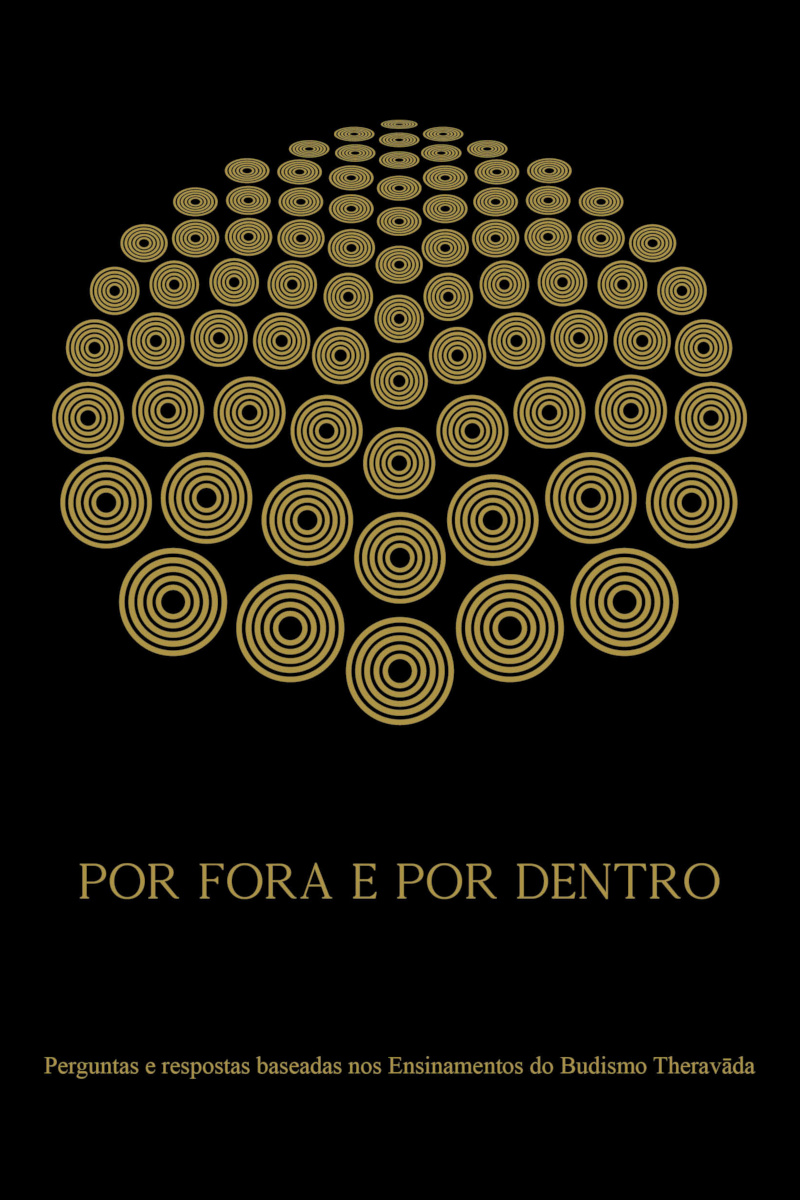
\includegraphics[width=\paperwidth]{./desktop-cover.jpg}}
\fi

\cleartorecto
\thispagestyle{empty}
\photoFullBleed{buddha-sun-Gr-crop.jpg}
\vspace*{4em}

{\centering
\ifoverleaf\relax%
\else%
  \color[gray]{1}%
\fi

\settowidth{\titleLength}{%
  {\vidalokaFont\fontsize{20}{20}\selectfont\thetitle}%
}

{\vidalokaFont\fontsize{20}{20}\selectfont\thetitle}\\[0.3\baselineskip]
\setlength{\xheight}{\heightof{X}}
\raisebox{0.5\xheight}{\rule{\titleLength}{0.25pt}}\\[0.3\baselineskip]
{\itshape
Perguntas e respostas baseadas nos\\ Ensinamentos do Budismo Theravāda
}

\vspace*{2em}

\theauthor

}



\cleartoverso
\thispagestyle{empty}

{\copyrightsize
\centering
\setlength{\parindent}{0pt}%
\setlength{\parskip}{0.8\baselineskip}%

Por Fora e Por Dentro

\emph{Perguntas e respostas baseadas nos\\
Ensinamentos do Budismo Theravāda}

por Ajahn Jayasāro

Publicações Sumedhārāma\\
\href{http://sumedharama.pt}{www.sumedharama.pt}

As publicações de Sumedharama são para distribuição gratuita.\\ 
Na maioria dos casos, isto é possível graças a doações, 
de indivíduos ou grupos,\\
feitas especificamente para que as publicações dos ensinamentos\\
do Buddha possam estar disponíveis gratuitamente.

\textit{Sabbadānaṃ dhammadānaṃ jinati}\\
`A oferta de Dhamma é superior a qualquer outra oferta.'

Este livro encontra-se disponível para distribuição gratuita em\\
\href{http://forestsangha.org/}{www.forestsangha.org}

ISBN \theISBN

Copyright \copyright\ Publicações Sumedhārāma 2019

Traduzido por Helena Gallis

Tradução autorizada da edição inglesa:\\
\emph{Without and Within}\\
Panyaprateep Foundation, 2015

\vfill

{\footnotesize

Este trabalho está licenciado com uma Licença Creative Commons\\
Atribuição-NãoComercial-SemDerivações 4.0 Internacional.

Veja página \pageref{copyright-details} para mais detalhes sobre direitos e restrições desta licença.

Produzido com o sistema tipográfico \LaTeX.\\
Fonte utilizada: Gentium, Vidaloka, Allura e Crimson~Roman.

\theEditionInfo

}}


% NOTE: Only for the Katannyuta print edition.
%\cleartorecto
\thispagestyle{empty}

\mbox{}\vfill

\begin{centering}
\itshape

{\upshape Dedicação}\\[0.4\baselineskip]
Gostaríamos de agradecer a todos aqueles que\\
ajudaram na preparação deste livro, em especial ao grupo\\
Kataññutā da Malásia, de Singapura e da Austrália,\\
por tornarem possível esta publicação para\\
distribuição gratuita em português.

\end{centering}

\vfill

\vspace*{6em}
\mbox{}


\chapterstyle{hightitle-toc}

\cleartorecto
\tableofcontents*

\chapterstyle{hightitle}

\cleartoverso
\photoFullBleed{birds-Gr-crop.jpg}

\cleartorecto
\chapter{Prefácio à edição portuguesa}

{\fontsize{10.5}{13.5}\selectfont

‘Por Fora e Por Dentro’ encontra-se disponível há já algum tempo na língua
portuguesa, em formato electrónico. Este ano, através da generosidade de
Buddhadasa Indapañño Archives (BIA), a versão impressa foi produzida como
Dhammadāna. Gostaria de expressar o meu apreço a todos aqueles que participaram
neste projecto, em particular a BIA e ao Mosteiro Budista Sumedhārāma.
Anumodanā!

‘Por Fora e Por Dentro’ oferece um vislumbre introdutório aos ensinamentos
Budistas, da forma como estes são interpretados e praticados na tradição Budista
Theravada encontrada na Tailândia. Possam os curtos sumários deste livro
inspirar os leitores a embarcar num estudo e prática mais profundos destes
maravilhosos e libertadores ensinamentos.

\bigskip

{\raggedleft
  Ajahn Jayasaro\\
  Janamara Hermitage\\
  Maio de 2020
\par}

}



\clearpage
\chapter{Prefácio}

{\fontsize{10.5}{13.5}\selectfont

A primeira edição deste livro foi impressa em 2013 de forma a celebrar três
ocasiões auspiciosas: os 2600 anos desde a iluminação do Buda, o 100º
aniversário de Sua Santidade Somdet Phra Sangharaja Chao Krom Luang
Vajirananasamvara (Charoen Savaddhano), o 19º Patriarca Supremo do Reino da
Tailândia, e o 84º aniversário de Sua Majestade Phrabat Somdet Phra Paraminthra
Maha Bhumibol Adulyadej (Rama IX). Foram distribuídas mais de 82.996 cópias da
primeira edição em 289 hotéis (em 39 províncias) e em bibliotecas, templos e
escolas, quer dentro quer fora da Tailândia.

Para celebrar o 10º aniversário da Buddhadasa Indapanno Archives Foundation
(BIA) in 2020, uma segunda edição foi publicada pela Fundação, em colaboração
com Ajahn Jayasaro e com a Panyaprateep Foundation. Para além do Inglês, a nova
edição, concisa e fácil de transportar, foi também traduzida em muitas outras
línguas, incluindo Chinês, Português, Russo e Francês.

Espera-se que a distribuição deste livro continue a beneficiar grandemente o
público, indo ao encontro das palavras do Somdet Phra Buddhaghosacariya (P.A.
Payutto): uma oferta de Dhamma que difundirá conhecimento, compreensão e sentido
de justiça, contribuindo para uma felicidade verdadeira e duradoura entre as
pessoas de todo o mundo.

``Por fora e Por Dentro'' irá essencialmente beneficiar quer os turistas na
Tailândia, quer as restantes pessoas do globo. Para além de enriquecer vidas,
este livro ajudará a nutrir as mentes e os corações dos leitores e proporcionará
uma noção de paz, bondade e clareza, tornando-o numa verdadeira oferta de
Dhamma, tal como foi projectado para ser.

\bigskip

{\raggedleft
  Buddhadasa Indapanno Archives Foundation (BIA)\\
  Fevereiro de 2020
\par}

}



% \clearpage
\chapter{Prefácio à primeira edição}

{\fontsize{10.5}{13.5}\selectfont

Cada religião tem as suas características específicas, e o Budismo não é
excepção. Cada país budista tem práticas diferentes o que por vezes pode ser
confuso para os visitantes. O objectivo deste livro é oferecer um esclarecimento
conciso das práticas budistas na Tailândia e ajudar os visitantes estrangeiros a
desfrutarem da sua vista. Se isto levar a uma melhor compreensão entre as
diferentes religiões e países, isso será uma bênção.

Ao longo dos anos houve muitas tentativas para haver livros sobre o Budismo nos
hotéis na Tailândia, mas nenhum deles se encontra actualmente disponível de uma
forma abrangente. Assim, a Buddhadasa Indapanno Archives Foundation (BIA),
iniciou este projecto em 2012, para celebrar os 2600 anos da Iluminação do Buda,
o centésimo aniversário da Sua Santidade Somdet Phra Nyanasamvara , o Patriarca
Supremo da Tailândia e o octogésimo quarto aniversário de Sua Majestade o Rei
Bhumibol Adulyadej.

Gostaríamos de agradecer aos seguintes contribuidores:

Crown Property Bureau, The Ministry of Culture, Siam Cement Group, Siam
Commercial Bank, Kiatnakin-Phatra Financial Group, Thai Hotel Association,
Tourism Authority of Thailand, Amarin Printing and Publishing Plc. e a
Panyaprateep Foundation.

Como qualquer outra publicação este livro passou por vários obstáculos e
revisões. Com o encorajamento do autor, Ajahn Jayasaro, bem como o apoio de
respeitáveis monges e leigos, foi-nos possível finalizar este livro com muita
alegria e pouca frustração. É para nós uma honra e uma experiência memorável
puder contribuir para esta importante causa.

{\raggedleft
  Buddhadasa Indapanno Archives Foundation (BIA)\\
  Banguecoque, Tailândia\\
  Agosto de 2013
\par}

}



% \clearpage
\chapter{Palavras de Agradecimento}

{\fontsize{10.5}{13.5}\selectfont

A publicação deste livro, cujo propósito é estar disponível em hotéis e outros
tipos de alojamento, vai ao encontro de uma necessidade de longa data. Outros já
haviam encetado este tipo de projecto mas acabaram sempre por o abandonar; assim
este livro vem finalmente colmatar uma falta importante. Ajahn Jayasaro
escreveu-o sob a forma de Perguntas e Respostas, tornando-o de fácil leitura e
sem um tom demasiado académico. Para além disso ele aplicou a sua vasta
experiência de estudo, ensino e prática budista, para seleccionar os tópicos
adequados. Ele observou e reflectiu quais os assuntos que são normalmente mais
relevantes e importantes de serem explanados.

Ele também aborda neste livro temáticas comummente mal interpretadas e outras
que contêm aspectos importantes e úteis, que são muitas vezes minimizados.
Assim, Ajahn Jayasaro escolheu temáticas adequadas nas quais ele responde às
necessidades dos interessados no Budismo, esclarece mal-entendidos e aponta para
áreas que requerem atenção. Explica e oferece conselhos, esclarecendo os
leitores sobre conceitos fundamentais do Budismo.

Há uma temática muito benéfica que impregna toda a expressão deste livro: o
elegante e meticuloso cultivo de tudo quanto de nobre existe no coração e na
mente

Aqueles que visitam países como a Tailândia encontram actividades, costumes,
tradições e comportamentos que reflectem o espírito Budista, e estes podem ser
intrigantes e fora do comum. Este livro ajudá-los-á a compreender melhor estas
experiências, podendo eles assim não só desfrutar das suas viagens, como também
terem uma aprendizagem de vida mais rica.

Pode haver leitores que estejam também a passar por um período mais difícil nas
suas vidas ou a viverem algum tipo de infelicidade e quiçá as compreensões e
realizações despoletadas por esta leitura possam ajudar a resolver algumas
dessas dificuldades.

Por último, quando os leitores se encontrarem de volta nos seus quartos de hotel
e procurarem descontrair, este livro pode ser um companheiro que nutre os seus
corações e as suas mentes. Ainda que somente aberto com o objectivo de relaxar,
poderá oferecer uma sensação de paz, bondade e clareza.

Eu gostaria de acrescentar o meu sincero agradecimento ao ‘Buddhadasa Indapanno
Archives’ pelo esforço e dedicação dos seus membros na publicação deste livro,
de forma a este poder estar disponível em hotéis e hospedarias. É uma oferta de
Dhamma que disseminará conhecimento, compreensão e integridade, contribuindo
para uma felicidade verdadeira e duradoura, partilhada por pessoas à volta do
mundo.

\bigskip

{\raggedleft
  Phra Brahmagunabhorn (P. A. Payutto)\\
  9 de Maio de 2013
\par}

}



\clearpage
\chapter{Introdução}

Para as pessoas que visitam a Tailândia não é fácil que as tradições
budistas, com que se deparam aqui, façam sentido. São poucos os guias
turísticos que sabem explicar os princípios do Budismo com bastante
clareza, e os amigos do Budismo Tailandês têm tendência a ser igualmente
vagos. Este livro pretende oferecer uma introdução aos ensinamentos do
Buda, o que lançará alguma luz num assunto que, para os não"-budistas,
pode parecer tão inesperadamente racional quão exoticamente estranho.

Este não é um livro habitual. Pretende ser tão conciso quanto possível,
e trata num parágrafo assuntos que se encontram tratados noutros livros
em centenas de páginas. É óbvio que se omitiu muita coisa. Aos leitores
interessados em saber mais sobre pontos específicos, é-lhes referido a
lista de recursos que se encontra no fim deste livro.

Ao longo dos últimos 2.600 anos, desenvolveram"-se muitas formas de
Budismo. Este livro trata apenas dos ensinamentos da tradição do Budismo
Theravāda, e em particular da forma do Theravāda da Tailândia (o que
difere em certos detalhes menores da sua expressão de outros países
Theravāda, tais como O Sri Lanka ou Burma). Este livro também foi
escrito sob a perspectiva de um monge particular, que vive dentro da
tradição Theravāda Tailandesa.

Nasci em Inglaterra, mas tenho vivido nos mosteiros da floresta e
ermitérios do nordeste da Tailândia desde 1978. Inevitavelmente, o meu
passado e prática influenciaram as interpretações que aqui se encontram.

\clearpage

Fui bastante afortunado por ter estudado com mestres sábios, e esta
apresentação do Dhamma deve muito a eles, em particular a dois dos
monges mais importantes da era moderna, o Venerável Ajahn Chah e Prha
Brahmagunabhorn (P.A.Payutto). Gostaria de deixar expressa a minha
profunda gratidão a ambos.

\bigskip

{\raggedleft
  Ajahn Jayasāro\\
  Ermitério Janamāra\\
  Março de 2013
\par}


\cleartoverso
\chapter{Cântico de Bênçãos}

\vspace*{-\baselineskip}

\begin{verse}

Evitar os tolos,\\
Associar-se aos Sábios,\\
E honrar quem é digno de honra.\\
Estas são as maiores bênçãos.

Viver em locais adequados,\\
Com os frutos das boas acções passadas,\\
Guiado pelo caminho correcto.\\
Estas são as maiores bênçãos.

Proficiente em estudos e ofícios,\\
Com disciplina sublimemente treinada,\\
E discurso verdadeiro agradável ao ouvido.\\
Estas são as maiores bênçãos.

Apoiar os pais,\\
Zelar pela família,\\
E ter uma vida inofensiva para os demais.\\
Estas são as maiores bênçãos.

Generosidade e uma vida honesta,\\
Oferecer ajuda a familiares e amigos,\\
Agir de forma que não promova remorsos.\\
Estas são as maiores bênçãos.

Resoluto a controlar-se, a abandonar os caminhos do mal,\\
Evitar intoxicantes que entorpeçam a mente,\\
E ser diligente em todas as ocasiões.\\
Estas são as maiores bênçãos.

Respeito e humildade,\\
Contentamento e gratidão,\\
Ouvir o Dhamma frequentemente ensinado.\\
Estas são as maiores bênçãos.

Paciência e vontade para aceitar as próprias falhas,\\
Visitar os respeitáveis buscadores da verdade,\\
E partilhar o Dhamma frequentemente.\\
Estas são as maiores bênçãos.

Dedicar-se ardentemente à Vida Santa,\\
Ver as Nobres Verdades directamente por si\\
E realizar o Nibbana.\\
Estas são as maiores bênçãos.

Ainda que em contacto com o mundo,\\
A mente mantem-se inabalável,\\
Perfeitamente segura além de toda a aflição.\\
Estas são as maiores bênçãos.

Aqueles que seguem este caminho,\\
Conhecem a Victória onde quer que vão,\\
E qualquer lugar para eles é seguro.\\
Estas são as maiores bênçãos.

{\raggedleft
Maṅgala Sutta, Sutta Nipāta 24
\par}

\end{verse}



\addtocontents{toc}{\addvspace{10pt}}

\mainmatter

\chapterPhotoTwoPageLeft{buddha-moon-Gr-crop}

\setlength{\chapterTitleTopSkip}{10mm}
\definecolor{photoChapterText}{gray}{1}

\chapterNote{%
  O Tathāgata é o Puro, o Perfeitamente Iluminado\\
  Ele é impecável na conduta e na compreensão,\\
  O Conhecedor dos Mundos:\\
  Ele treina com perfeição todos aqueles que querem ser treinados;\\
  É o Professor de deuses e de humanos;\\
  É o Desperto e Santo.%
}

\chapter{O Buda}

\chapterPhotoTwoPageRight{buddha-moon-Gr-crop}

\section{Quem era o Buda?}

Há 2.600 anos nasceu uma criança na família real do clã Sakyan, um povo
que vivia no nordeste da Índia e que agora fica na fronteira do Nepal.
Foi"-lhe dado o nome de Siddhattha. Com 29 anos, o Príncipe Siddhattha
renunciou à vida de facilidades e privilégios em busca da libertação
espiritual. Seis anos depois, após uma memorável noite de meditação,
sentado de pernas cruzadas sob uma árvore bodhi, realizou `o
inexcedível despertar pleno'. Ao fazê"-lo, tornou"-se `O Buda', `O
Desperto'.

No seguimento do seu despertar, o Buda dedicou os restantes quarenta e
cinco anos de sua vida a revelar o Dhamma: a verdadeira realidade, bem
como o caminho conducente à realização dessa verdade. Durante esse
tempo, estabeleceu uma ordem monástica (Sangha) para os seus discípulos,
homens e mulheres, que queriam deixar as tarefas mundanas e devotarem"-se
com todo o seu ser ao estudo e à prática dos seus ensinamentos.

\section{O que é a iluminação?}

A iluminação refere"-se à libertação do sofrimento e das aflições mentais
ou `obstáculos' que são a sua causa. É a realização da própria
natureza de `como as coisas são'. Um ser iluminado compreende a
natureza condicionada dos fenómenos impermanentes e vivencia o
Nibbāna,\footnote{%
  `Nibbāna' em Pali é o mesmo que `Nirvana' em Sânscrito.}
a realidade incondicionada subjacente. O Buda referia"-se a este estado
como a `felicidade suprema'. A mente iluminada caracteriza"-se pela
sabedoria, compaixão e pureza. O Buda ensinou que todos os seres
humanos, masculinos e femininos, nascem com o potencial da iluminação.

O Buda falou dos quatro estádios de iluminação, e consequentes quatro
tipos de seres iluminados. O primeiro destes seres é `o que entra na
corrente', o segundo `o que volta uma vez', o terceiro `o que não
volta', e o último é o totalmente iluminado `o \emph{arahant}'. O
alcançar destes estados depende da prática do Óctuplo Caminho enunciado
pelo Buda. O seu resultado é assinalado pelo total desaparecimento na
mente de certos estados mentais confusos. Já não é possível regressar a
partir de tal estado. Aquele que alcança o primeiro estádio de
iluminação deve assegurar"-se de alcançar o estádio final no prazo máximo
de sete vidas. Ele, ou ela, entrou na corrente que conduz
irrevocavelmente ao oceano do Nibbāna.

\section{O que significa `Buda'?}

A palavra Buda significa `o que despertou'. O Buda ensinou que o ser
humano não iluminado vive num estado que pode ser comparado a estar a
dormir, ou a um sonho. Através da clara luz da sabedoria, e sem qualquer
ajuda, o Buda foi aquele que despertou desse sonho, para a verdadeira
natureza da existência. Guiado pela compaixão, o Buda é aquele que
procurou partilhar a sua compreensão da via do despertar, com todos os
seres que desejaram seguir as suas pisadas.

\section{O Buda era um ser humano?}

O Príncipe Siddhattha era um ser humano. Na noite em que realizou a
suprema iluminação, tornou"-se um Buda, e a partir desse momento, nunca
mais foi um ser humano, na acepção comum do termo. Para os olhos dos
não"-iniciados, o Buda poderá ter parecido como um forte líder religioso
carismático, alguém que teve uma morte normal aos oitenta anos. Contudo,
aqueles com faculdades mais desenvolvidas aperceberam"-se de que não
havia qualquer aparência externa, nem quaisquer palavras, conceitos, ou
categorias que servissem para \mbox{exprimir} a maravilhosa natureza imortal da
sua natureza de Buda.

\section{Que provas há da existência de Buda?}

\begin{enumerate}
\item
  Evidências arqueológicas fornecem fortes provas empíricas de Buda,
  enquanto figura histórica.
\item
  Muitos dos mosteiros e cidades mencionados nos discursos de Buda
  puderam ser localizados.
\item
  As relíquias de Buda foram recuperadas de locais mencionados nos
  textos.
\item
  O imperador budista Asoka, independentemente da data, esculpiu
  inscrições em colunas de grés que erigiu ao longo de todo o seu vasto
  império -- alguns dos quais sobreviveram até hoje -- referindo"-se
  extensivamente ao Buda.
\item
  Há muitas evidências circunstanciais nos primeiros textos.
\item
  A coesão e ausência de contradição interna nos discursos de Buda,
  juntamente com as prescrições finamente detalhadas para a ordenação do
  corpo monástico encontradas nos `Livros da Disciplina', apontam
  seriamente para um autor único.
\item
  Claro que a evidência física e a lógica sempre deixam espaço para a
  dúvida. Numa ocasião, o Buda disse: `Quem vê o Dhamma, vê"-me a mim'.
  Por outras palavras, a verificação da verdade dos ensinamentos na vida
  de cada um, é, sob o ponto de vista budista, a confirmação mais fiável
  da existência de Buda.
\end{enumerate}

\section{O Buda possuía poderes psíquicos?}

O Buda possuía imensos poderes psíquicos extraordinários. Os poderes
psíquicos podem (mas nem sempre) resultar de um treino intensivo da
mente, e ainda hoje, existem praticantes de meditação que possuem tais
poderes. O Buda usava os seus poderes psíquicos com moderação,
normalmente como auxílio nos ensinamentos, quando outros métodos
provavam ser ineficazes; o exemplo mais conhecido ocorreu no encontro
com o notório assassino, Angulimala. O Buda considerou que a fé das
pessoas obtida com a visão de `milagres' vulgarmente afastava"-as mais do
caminho da sabedoria, do que as aproximava. Por esta razão, proibiu os
monges com poderes psíquicos de os revelarem aos leigos. A posse de
poderes psíquicos pode"-se tornar viciante. O Buda recomendou que os seus
discípulos não os considerassem como fins em si na vida espiritual.

\section{Quantos Budas há?}

De acordo com a tradição Theravāda, só pode haver um Buda de cada vez.
Contudo, existiram outros Budas no passado longínquo, e existirão mais
futuramente. O intervalo entre a aparição dos Budas é medido em
\emph{kalpas}. Um \emph{kalpa} é uma medida de tempo extraordinariamente
longa. O Buda forneceu esta definição:

\begin{verse}
Supõe, bhikkhu, que existia uma enorme montanha de pedra com
dez milhas de comprimento (uma yojana), dez milhas de largura e dez
milhas de altura, sem buracos nem fendas, uma massa sólida de pedra. Ao
fim de cada cem anos um homem bateria nela com um pedaço de pano
delicado. Essa enorme pedra poderá ser gasta e eliminada através desse
esforço, mas ainda assim o kalpa não terá chegado ao fim.

{\raggedleft
  Saṃyutta Nikāya, 15.5
\par}
\end{verse}

\section{Como era a relação de Buda com a sua família?}

O Buda demonstrou apreço pela sua família sob a forma que lhe era mais
adequada como Buda: conduzindo os seus membros para a via do despertar.
No primeiro ano após a sua iluminação, sete anos depois de se ter ido
embora, o Buda voltou à sua casa de origem na cidade de Kapilavatthu.
Esta visita viria a ter um profundo impacto, não apenas em todo o reino
Sakyan, mas mais ainda no seu pai, o rei Suddhodana; como resultado da
sua primeira visita, o rei realizou os dois primeiros níveis de
iluminação. Alguns anos mais tarde o Buda, apercebendo"-se da aproximação
da morte de seu pai, visitou o velho rei pela última vez e conduziu"-o ao
estado de arahant, o estado de iluminação mais elevado. Esta visita a
Kapilavatthu foi também notável pelo primeiro encontro com o seu filho
de sete anos, Rāhula, durante o qual o jovem requereu a sua herança.
Como resposta o Buda permitiu que ele se juntasse ao Sangha, como o
primeiro rapaz noviço.

O Buda não conseguiu ensinar a sua mãe em Kapilavatthu, uma vez que ela
tinha morrido ao dar à luz (a lenda conta que mais tarde ele a foi
ensinar no reino celestial onde ela residia); contudo, conseguiu ensinar
a sua madrasta e tia, Pajāpati. Foi ela quem requereu formalmente ao
Buda que fundasse uma ordem de monjas, e quando obteve o consentimento,
ela tornou"-se a sua líder mais sénior. A primeira geração de monjas
incluía muitas mulheres da família de Buda, incluindo a sua ex"-mulher
Yasodhara. Conta"-se que Pajāpati, Yasodhara e o filho de Buda, Rāhula,
todos eles atingiram o mais elevado estádio de iluminação.

\enlargethispage{\baselineskip}

Muitos dos parentes masculinos foram ordenados como monges e alguns
deles foram mencionados como tendo sido os seus discípulos mais
excepcionais. Entre eles estão Anuruddha, Nanda, e o mais famoso, o seu
companheiro de longa data, Ānanda.

\section{O Buda tinha sentido de humor?}

O Buda sabia que o sentido de humor, usado criteriosamente, pode levar à
verdade através de meios encantadores e que desarmam as pessoas. De vez
em quando, a sagacidade e o dom de discurso que o Buda tinha
desenvolvido ao longo da sua educação real vinham à tona nos seus
discursos com efeitos divertidos. Trocadilhos, reformulação brilhante de
termos, parábolas bizarras, e analogias cómicas podem ser encontrados
nos seus ensinamentos. Embora não exista nada em seus discursos que
evoque risos declarados no leitor moderno, ao ler algumas passagens,
poderão imaginar facilmente as faces do público de Buda engalanadas com
largos sorrisos.

\chapterPhotoTwoPageLeft{dhamma-hills-Gr-crop}

\chapterPhotoTwoPageRight{dhamma-hills-Gr-crop}

\setlength{\chapterTitleTopSkip}{10mm}
\definecolor{photoChapterText}{gray}{0}

\chapterNote{%
  O Dhamma foi bem apresentado pelo Abençoado,\\
  Aparente aqui e agora,\\
  Intemporal,\\
  Encorajando à investigação\\
  Conduzindo para a frente,\\
  A ser experimentado pelo sábio.
}

\chapter{O Dhamma}

\section{O que significa `Dhamma'?}

O Dhamma\footnote{`Dhamma' em Pali é o mesmo que `Dharma' em Sânscrito.}
refere"-se a:

\begin{enumerate}
\item
  A verdade das coisas, `como as coisas são', a verdadeira realidade.
\item
  Os ensinamentos do Buda que iluminam essa verdade, e que pormenorizam
  o caminho conducente à sua experiência directa.
\end{enumerate}

\section{O que são as Quatro Nobres Verdades?}

Todos os ensinamentos do Buda estão englobados no que se chama as Quatro
Nobres Verdades, e segundo ele explicou, tal como a pegada de qualquer
animal da floresta cabe dentro da pegada de um elefante. Estas verdades
revelam o problema fundamental da nossa existência, bem como a sua
resolução.

\begin{enumerate}[topsep=0pt]
\item Existe \emph{dukkha}
\end{enumerate}

Dukkha é geralmente traduzido como `sofrimento', mas na verdade tem um
significado bem mais profundo do que o que está implicado nessa palavra.
Dukkha refere"-se à insatisfação crónica da existência não iluminada.
Cobre todo o espectro da experiência, desde severas dores físicas e
emocionais até ao mais subtil sentido de desconforto e de carência.

\begin{enumerate}[resume,topsep=0pt]
\item Há uma causa para dukkha
\end{enumerate}

Dukkha não é uma dificuldade humana inalterável. Depende de certas
causas e condições, em particular dos desejos que surgem de uma
percepção fundamentalmente errada da nossa natureza humana.

\begin{enumerate}[resume,topsep=0pt]
\item Existe a extinção de dukkha
\end{enumerate}

Existe um fim total de dukkha, um estado de libertação e de verdadeira
felicidade.

\begin{enumerate}[resume,topsep=0pt]
\item Existe o caminho conducente à cessação de dukkha
\end{enumerate}

Através do cultivo do Óctuplo Caminho, dukkha é compreendido, as suas
causas são abandonadas e ocorre o seu término. Esta via envolve uma
educação ou uma prática em todos os aspectos da nossa vida, tanto no
interior como no exterior. Os oito factores são os que seguem:

\begin{enumerate}
\item Entendimento correto
\item Pensamento correcto
\item Discurso correcto
\item Acção Correcta
\item Meio de Subsistência Correcto
\item Esforço Correcto
\item Consciência Correcta
\item Concentração Correcta
\end{enumerate}

\section{Por favor explique mais detalhadamente o que é o Óctuplo Caminho.}

O Óctuplo Caminho é a educação holística, ou o treino do corpo, da fala
e da mente, que culmina no despertar.

O Entendimento Correcto refere"-se às crenças, visões, ideias, valores
que estão em harmonia com a forma como as coisas são. Inicialmente os
seus elementos mais importantes são a confiança na 1) capacidade humana
para se iluminar e 2) lei do kamma.\footnote{`Kamma' em Pali é o mesmo que `karma' em Sânscrito.}

O Pensamento Correcto refere"-se aos pensamentos consistentes com a Visão
Correcta. Caracterizam"-se por uma ausência de pensamentos indesejáveis,
em particular os do tipo 1) sensual, 2) hostil, ou 3) cruel. O
Pensamento Correcto inclui a aspiração de se libertar de todas as
aflições interiores, e alcançar pensamentos de bondade e compaixão.

O Discurso Correcto é um discurso verdadeiro, útil e intemporal, cortês
e gentil na sua intenção. É um discurso livre de 1) mentira, 2) rudeza,
3) calúnia e 4) maledicência.

A Acção Correcta refere"-se a acções que não prejudicam o próprio nem os
outros. Basicamente tem que ver com abster"-se de 1) matar, 2) roubar e
3) ter má conduta sexual.

O Meio de Subsistência Correcto significa sustentar"-se de forma a não se
prejudicar a si próprio, nem aos outros. Más formas de ganhar a vida,
enunciadas nos textos, incluem vender: 1) armas, 2) seres humanos, 3)
carne e peixe, 4) drogas e 5) venenos.

O Esforço Correcto refere"-se a tentar:

\begin{enumerate}[topsep=0pt,parsep=0pt]
\item Evitar que cheguem à mente pensamentos e emoções inadequados.
\item Reduzir e erradicar pensamentos e emoções inadequados que já tenham chegado à mente.
\item Introduzir antecipadamente na mente pensamentos e emoções adequados.
\item Manter e desenvolver pensamentos e emoções adequadas, já presentes na mente.
\end{enumerate}

A Consciência Correcta refere"-se a manter uma consciência alerta, serena
e confiante, no momento presente, em particular:

\begin{enumerate}[topsep=0pt,parsep=0pt]
\item No corpo humano
\item Sob o aspecto em que afecta a experiência: agradável, desagradável ou neutro.
\item No estado mental
\item Nos fenómenos mentais, em como se relacionam com o caminho para o despertar de Buda.
\end{enumerate}

A Concentração Correcta refere"-se à estabilidade interior, à clareza e à
paz experimentada nos quatro estádios da `absorção meditativa', ou `jhāna'.

O primeiro jhāna é caracterizado pelos cinco `factores jhāna': uma
sustentada atenção inicial, manutenção da atenção no objecto de
meditação, entusiasmo, felicidade, e focagem da mente. Consoante a mente
se torna mais refinada, os factores mais densos de jhāna desvanecem"-se.
O segundo jhāna é alcançado com o esvanecer da atenção inicial. Ao
desaparecer o entusiasmo assinala"-se o atingir do terceiro jhāna. Com a
perda da felicidade, a mente entra no quarto e mais subtil estado de
jhāna, que se distingue pela inabalável equanimidade.

\section{O que significa `tomar refúgio'?}

A vida é cheia de dificuldades, nunca está liberta de sofrimento, ou
pelo menos da possibilidade de este surgir. Ao sentirem"-se inseguros, e
num estado crónico de carência, os seres humanos desejam ardentemente
segurança. Alguns procuram"-na adoptando um sistema de crença ou o
conforto de rituais. Igualmente popular é o caminho das distracções:
perseguindo prazeres sensoriais, riqueza, fama, poder e estatuto. Sob o
ponto de vista budista nenhuma destas estratégias atinge esse alvo. Nem
os prazeres dos sentidos, nem o sucesso mundano poderão satisfazer as
necessidades humanas mais profundas. A fé nos dogmas ou a realização de
rituais não conseguem providenciar um refúgio verdadeiro. Enquanto as
pessoas não obtiverem clareza na compreensão de suas vidas e continuarem
a agir com pouca sensatez, nunca se sentirão em segurança.

Tomar refúgio na `Jóia Tripla' (Buda, Dhamma, Sangha) considera"-se
ser o primeiro passo para alcançar a libertação do sofrimento, bem como
das suas causas, pois fornece, aos esforços feitos pelos budistas, uma
base de suporte e uma direcção para alcançarem esse objectivo. O acto de
se refugiarem assinala o primeiro passo de compromisso no caminho do
Buda. Os budistas afirmam refugiar"-se no Buda, como seu professor e
guia, no Dhamma, os ensinamentos, como seu caminho, e no Sangha, os
discípulos iluminados, como sendo a inspiração para o caminho.

\section{Porque é que os ensinamentos budistas são referidos frequentemente como
  o Caminho do Meio?}

O `Caminho do Meio' é um termo usado pelo Buda em dois contextos
distintos. Primeiro, como característica"-cerne de seu ensinamento --
todas as coisas surgem e desaparecem devido às causas e condições --
como um caminho do meio entre os extremos do aniquilacionismo (a crença
de que tudo termina com a morte) e a do eternalismo (a crença que a
morte é seguida de felicidade ou de condenação eternas).

Segundo, o Buda apresentou o Óctuplo Caminho como um caminho médio entre
os extremos da indulgência sensorial e do vazio asceticismo, (`sem dor
não há benefício'). Contudo, seria um erro olhar para isto como sendo
apenas um ensinamento de moderação. Pelo contrário, o Caminho do Meio
deve ser compreendido dentro do conceito do esforço geral que leva ao
abandono dos estados mentais inadequados, ao cultivo dos estados mentais
adequados, e à libertação da ignorância e da ilusão. O Caminho do Meio
não se encontra ao se buscar um ponto médio entre os dois extremos, mas
antes, encontra"-se sempre presente naquilo que qualquer prática
espiritual possibilita como uma progressão excelente para o despertar.

\section{O que é que o Budismo ensina sobre a natureza da felicidade?}

Os seres humanos podem obter dois tipos de felicidade: a que depende dos
estímulos externos, a que não depende disso. O primeiro tipo de
felicidade é vivido, ao seu nível mais básico, nos prazeres sensoriais:
vendo, ouvindo, cheirando, saboreando e tocando coisas agradáveis.
Também inclui as emoções positivas que vivemos através das relações
pessoais, realizações mundanas e do estatuto social.

O segundo tipo de felicidade é conhecido com o desenvolvimento
espiritual. Inicialmente é desfrutado pelo cultivo da generosidade e da
disciplina moral, mas atinge os seus níveis mais profundos com a
meditação. Meditadores experientes reconhecem o entusiasmo e a
felicidade que acontecem numa mente focada, como sendo
inquestionavelmente superiores aos prazeres que dependem dos sentidos
mais densos. Mas os estados meditativos mais refinados não representam a
felicidade suprema. É no gradual abandono dos estados mentais nocivos --
a causa original do sofrimento -- que o praticante descobre um sentido
estável e sublime de bem"-estar. Isto é considerado como sendo um estado
superior de felicidade, experienciado como uma expressão natural de uma
mente refreada, mais do que como uma experiência de passagem sujeita a
ganhos ou perdas.

Os budistas leigos são encorajados a procurar, moderadamente, a
felicidade no mundo, compatível com o acesso à felicidade interior; e a
renunciar à complacência dos prazeres mundanos, que distraem a mente do
trabalho espiritual.

\section{Porque é que tão poucas pessoas parecem ser verdadeiramente felizes?}

O Buda ensinou que todos os seres vivos nascem com um desejo instintivo
de evitar o sofrimento e de vivenciar a felicidade. O problema é que,
por ausência da sabedoria, continuamos a agir criando condições para
sofrer, bem como negligenciando as acções que criariam as condições para
sermos felizes. Procuramos a felicidade nas coisas que inevitavelmente
nos vêm a desapontar; evitamos o que nos conduziria a um bem"-estar
duradouro. Em resumo, somos o nosso pior inimigo.

São poucas as pessoas que consideraram seriamente a natureza da
felicidade. Daqueles que o fizeram, ainda menos são as que se
comprometeram a erradicar sistematicamente os seus obstáculos internos e
a cultivar as condições que a suportam. Não é de surpreender que tão
poucas pessoas sejam verdadeiramente felizes.

Uma das premissas básicas do Budismo é a de que quanto mais claramente
virmos a natureza das coisas, menos sofreremos, e mais felizes seremos.
Na verdade, o Buda referiu"-se ao \emph{Nibbāna}, o objectivo da prática
budista, como a `suprema felicidade'. A felicidade mundana é fugaz e
nada fiável. A felicidade de uma mente controlada é um refúgio
duradouro.

\section{Os budistas falam muito do momento presente. Isso não entra em conflito
  com o que se aprende nas experiências passadas, ou com planear o futuro?}

O passado e o futuro encontram"-se no momento presente: o passado como
memória, o futuro como pensamento e imaginação. Qualquer acesso a
experiências passadas, qualquer decisão relativa ao futuro é actividade
mental que ocorre inevitavelmente no momento presente -- não há escolha,
é tudo quanto temos. O problema é que ao não se estar consciente da
memória, como memória, e do pensamento, como pensamento, facilmente
perdermo"-nos neles. Quando perdemos a presença de espírito desta
maneira, a nossa vida torna"-se uma abominável sombra de si própria.

Quanto mais conscientes estivermos do momento presente, menos confusa se
torna a mente, e mais fácil se torna aprender com as experiências
passadas, e planear o futuro com sabedoria.

\section{O que é o mérito?}

O mérito (\emph{puñña}) significa a purificação interna que ocorre por
acções virtuosas do corpo, das palavras e da mente. As acções meritórias
elevam e enobrecem a mente, e são acompanhadas por um sentimento de
bem"-estar.

Na Tailândia, a expressão popular de `criar mérito' (\emph{tham boon)}
refere"-se geralmente à contribuição de ofertas para a ordem monástica.
Tais ofertas, quando dadas com a motivação certa, podem efectivamente
ser meritórias, mas o mérito não se restringe apenas a esses actos.

As acções generosas são valiosas porque reduzem o poder do apego
egoísta, e ensinam a alegria da dádiva. Praticar os preceitos é
meritório porque enfraquece o impulso de nos magoarmos e de magoar os
outros, porque habitua a mente a libertar"-se de remorsos e a sentir
respeito por si próprio. Mas o tipo de mérito mais importante vem da
prática do Óctuplo Caminho, particularmente da prática da meditação.
Meditar com regularidade implica comprometer"-se no cultivo das
competências da vida. Significa responsabilizar"-se directamente pelo
abandono das causas do sofrimento, e por exponenciar a paz, a sabedoria
e a compaixão. Como a meditação é que efectua a maior transformação da
mente, ela é o mais portentoso gerador de mérito.

O Buda ensinou que os frutos do mérito não terminam na morte, mas
contribuem para um bom renascer. Embora o Buda enfatize a importância da
libertação do ciclo do nascimento e da morte (saṃsāra), também reconhece
que, para aqueles que não estão preparados para tal caminho, a
acumulação de mérito como benefício desta e doutras vidas futuras é uma
via compreensível (e nada pouco inteligente) a seguir.

\section{Por vezes afirma"-se que o Budismo é uma ciência. O~que é que isso
  significa?}

Existem semelhanças entre as práticas contemplativas budistas e o método
científico, na rejeição da fé cega e na ênfase da investigação imparcial
dos fenómenos, essencial a ambos métodos de investigação. Contudo,
também há diferenças. Nas suas investigações, a ciência limita"-se a
estudar tudo quanto é publicamente verificável, possível de medir, e que
pode ser repetido sempre que se deseja. A investigação introspectiva
levada a cabo pelos praticantes de meditação budistas não o é.
Actualmente a maioria dos cientistas assumem, como premissas básicas do
seu trabalho, um número de asserções não comprovadas, com as quais os
budistas não concordam. A mais notável destas é a crença que a mente é
um fenómeno meramente criado pelos trabalhos do cérebro.

As hipóteses e as teorias surgem na mente humana - não são embebidas no
mundo externo. A experiência subjectiva é a característica principal da
nossa vida. A contenda budista defende: qualquer busca das verdades
perpétuas que ignore este facto, ficará para sempre votada ao sucesso
parcial.

Apesar destas e doutras diferenças entre o Budismo e a ciência, há que
reconhecer que muitos budistas sentem que os seus pontos de vista estão
em maior consonância com os dos cientistas seculares, do que com a visão
da maioria das outras tradições religiosas.

\section{Será o Budismo uma religião pessimista?}

Pessimismo, numa acepção mais comum, significa `uma tendência para ver
o aspecto pior das coisas, ou acreditar que vai acontecer o pior; uma
falta de esperança ou de confiança no futuro', e sob uma perspectiva
filosófica: `uma crença de que este mundo é tão mau como deveria de
ser, ou de que o mal, em última instância, prevalecerá sobre o bem'.

Nenhum destes significados se aplica aos ensinamentos budistas. O Buda
ensinou que tudo quanto surge desaparece de acordo com as causas e as
condições. Se, numa determinada situação, prevalecerem as causas e as
condições para que aconteça o pior, então o pior acontecerá; se
prevalecem as causas e as condições para que aconteça o melhor resultado
possível, então surgirá o melhor desfecho. Ele enfatizou que se deve
aprender a ver tudo com clareza, em vez de se adoptarem atitudes
unilaterais.

O Buda, ao compreender a natureza causal dos fenómenos, não postulou
valores absolutos de bem e de mal, opondo"-se entre si numa guerra sem
fim. Por isso, há que descartar a ideia de ele ter ensinado o triunfo
final de um dos lados da luta, coisa que, primeiro de tudo, ele não
reconheceu existir. Os budistas defendem que, se uma chávena de chá
tiver um sabor salgado, mesmo que seja o mais desagradável possível, não
é uma evidência de um universo essencialmente maligno. É simplesmente o
resultado de alguém que se enganou no recipiente, pegando no do sal, em
vez do açúcar.

\section{Mas afinal o Budismo não trata só do sofrimento?}

O Buda disse que, todos os seus ensinamentos, tradicionalmente contados
como 84.000, se poderiam reduzir a apenas dois: sofrimento e o fim do
sofrimento. O sofrimento, no sentido de aflição física ou mental, é só a
expressão mais grosseira de dukkha. A relação que existe entre a palavra
`sofrimento', em Inglês (e em Português), e o conceito de dukkha,
em Pāli, pode ser vista como a comparação entre vermelho vivo e cor.
Dukkha também pode ser traduzido como um sentido crónico de ausência, ou
como um defeito, ou incompletude de experiência. Neste sentido, dukkha é
experiência vista como `não"-Nibbāna'. Por este motivo, até mesmo os
estados mentais mais sublimes ainda são considerados como existindo no
domínio de dukkha, porque como são fenómenos condicionados, o apego que
se lhes tem não deixa que aconteça a derradeira paz.

Posto de uma forma mais simples, dukkha pode ser expresso como `uma
ausência de verdadeira felicidade'.

O Buda ensinou a via para a cessação do sofrimento, mas enfatizou que a
libertação do sofrimento só seria possível, se ele fosse confrontado e
completamente compreendido na sua natureza. Na Primeira Nobre Verdade, o
Buda afirma que a vida do ser comum não iluminado se caracteriza por
dukkha, devido aos anseios que acompanham o desconhecimento de como as
coisas são.

\section{É correcto dizer que o Budismo nos ensina a renunciar a todos os
  desejos?}

O Budismo distingue dois tipos de desejos: o primeiro (tanhā), a ser
abandonado, e o segundo (chanda), a ser cultivado.

Tanhā é o desejo que surge de um mal"-entendido básico sobre como são as
coisas: o facto de se ver permanência, felicidade e individualidade,
onde não existem. O desejo pelos prazeres, a obter através de posse, de
descartar algo, e de se tornar em algo, é tanhā. Tanhā leva ao
sofrimento pessoal e é a base de quase todos os males sociais.

Chanda é o desejo que surge de uma compreensão correcta de como as
coisas são. No seu cerne reside a aspiração à verdade e ao bem. O desejo
de fazer bem, de actuar bem, de agir com bondade, de agir com sabedoria
-- todos os desejos baseados na aspiração à verdade e ao bem conduzem à
realização pessoal e a sãs comunidades.

A distinção entre chanda e tanhā não é filosófica, mas psicológica. Ao
se observar de perto a crua experiência de vida, a distinção entre
desejos que levam à felicidade genuína, e os que não levam, torna"-se
cada vez mais clara.

\section{O que significa `largar'?}

O Buda ensinou"-nos a observar como nós criamos sofrimento constantemente
para nós próprios, apegando"-nos ao corpo e seus sentidos, aos
sentimentos, percepções, pensamentos, emoções, como sendo `eu' ou `meu'.
Aprender a abandonar esse hábito, é aprender a `largar'. Tal não é
possível por um acto de vontade. O acto de largar ocorre naturalmente
quando a mente treinada se torna suficientemente acutilante para se
aperceber que não existe nada na experiência directa que possa
corresponder ao conceito de `eu' e `meu'.

`Eu' e `meu' não são, contudo, meras ilusões; são convenções sociais
extremamente úteis, e o Buda ensinou a respeitá"-las como tal. Embora o
corpo, por exemplo, estritamente falando seja `não meu', não quer dizer
que deva ser negligenciado. Largar o corpo não significa que se deva
deixar de praticar exercício, de tomar banho ou de ter uma dieta
saudável. Significa não permitir que a vida seja definida em termos
corporais. Significa libertar"-se de toda a ansiedade, insegurança e
vaidade, de todo o medo de envelhecer, adoecer, e morrer, que acompanham
uma relação nada sábia com o corpo.

`Largar' é também um termo usado para um esforço inteligente. Ao
sabermos que nenhum esforço que façamos existe em vão, que será sempre
afectado de alguma forma pelas condições sobre as quais não temos
controlo, largamos as nossas exigências e expectativas relativas ao
futuro. Criamos as melhores condições possíveis para atingir os nossos
objectivos, e depois, libertamo"-nos dos resultados.

\section{Como é que alguém se torna budista?}

Falando de forma prática, alguém torna"-se budista quando, ao se refugiar
no Buda, no Dhamma, e no Sangha, começa a aplicar"-se no estudo e a
aplicar os ensinamentos de Buda na sua vida.

Nos países budistas, como a Tailândia, nunca houve cerimónias
específicas, onde as pessoas possam afirmar formalmente a sua devoção ao
Budismo. De certa forma, talvez isto se deva por o Budismo não ser uma
religião baseada na adopção de determinadas crenças; e, em parte, também
por não existir qualquer proselitismo budista, poucos são os
recém"-convertidos. Para o melhor e para o pior, as pessoas encaram a sua
identidade budista como algo garantido, assumindo que são budistas desde
o dia em que nasceram.

A situação é algo diferente na Índia. Aproximadamente nos últimos
setenta anos, um grande número de Dalit (antes chamados de `intocáveis')
converteram"-se ao Budismo seguindo o exemplo do seu líder Dr. Ambedhkar.
Levaram"-se a cabo imensas cerimónias de conversão, onde se formalizou a
aceitação dos refúgios em Buda, Dhamma e Sangha, e um compromisso de
viver de acordo com os cinco preceitos. (Esta fórmula de requerer os
refúgios e os preceitos a partir da comunidade monástica é incorporada
em quase todas as cerimónias budistas na Tailândia.)

\section[O que são conta\kern-0.1pt minações?]{O que são contaminações?}

A mente destreinada é presa de vários estados mentais que arruínam o seu
esplendor natural. Estes incluem as diversas formas de cobiça, inveja,
raiva, ódio e animosidade, entorpecimento e agitação, complacência,
confusão, arrogância, desprezo e preconceito, e apego cego a pontos de
vista e crenças. Felizmente, nenhum destes estados mentais está
irrevogavelmente conectado à mente; qualquer um pode ser eliminado pela
prática do Óctuplo Caminho. Estes estados mentais negativos e
prejudiciais são chamados `\emph{kilesa}', na língua Pāli, geralmente
traduzidos como `contaminações ou corrupções'.

Neste livro a expressão `aflições mentais' tem sido preferida a
`contaminações'. As razões desta interpretação não ortodoxa deve"-se, em
primeiro lugar, ao facto de as contaminações serem geralmente entendidas
como sendo irreversíveis, mas as kilesa, não o são; em segundo lugar,
porque `aflições mentais' é um termo actual e poderoso que ilumina as
atitudes descuidadas tendo em vista kilesa; em terceiro lugar, porque
admite a gradação: podemos falar de algo com sendo levemente aflitivo, e
de algo muito aflitivo.

\section{O Budismo é uma religião ou uma filosofia?}

O Budismo pode ser desconcertante para algumas pessoas educadas dentro
de algumas grandes tradições monoteístas, tais como o Cristianismo ou o
Islamismo. Embora as tradições budistas tenham espaço para a devoção e a
cerimónia, o Budismo não tem dogmas, nem uma escritura única. Não
envolve adoração a um deus. O que o Budismo tem é um conjunto de
ensinamentos, que noutras tradições seria considerado dentro do domínio
da filosofia e da psicologia. Por este motivo têm existido muitas
dúvidas se o Budismo é uma religião, ou não.

O Budismo não se configura, de modo algum, no molde de religião criado
no mundo ocidental; se tal significa que o Budismo não é de modo algum
uma religião, ou se é simplesmente um tipo diferente de religião, é um
assunto em debate. Ao colocar o argumento na segunda possibilidade,
pode"-se dizer que, não obstante as religiões que se desenvolveram no
Médio Oriente sejam essencialmente sistemas de crenças, o Budismo é um
sistema educativo.

\section{Existem algumas escrituras budistas?}

O Tipițaka (literalmente, `os três cestos') é uma colecção de textos
fundamentais do Budismo Theravāda preservados na antiga língua da Índia,
o Pāli. Na tradução inglesa os Tipițaka cobrem à volta de 20.000 páginas
impressas. Os Tipițaka dividem"-se em três secções:

\textbf{O Vinaya Piṭaka}\\
A colecção de textos contendo o código disciplinar para monges e monjas,
e as instruções para gerir os assuntos monásticos. As últimas incluem,
por exemplo, as secções de etiqueta monástica, cerimónias e a relação
correcta a ter com os `quatro bens essenciais': a indumentária, a
comida da mendicância , o local de residência e os remédios, bem como os
procedimentos para a ordenação de novos membros, e a resolução de
disputas.

\textbf{O Sutta Piṭaka}\\
A colecção de suttas, ou discursos. Inclui todos os ensinamentos
registados que o Buda ensinou de Dhamma, juntamente com um pequeno
número de discursos dados pelos seus discípulos. O Sutta Pițaka está
dividido em cinco Nikāyas, ou colecções:

\begin{packeditemize}
\item Dīgha Nikāya -- a `colecção dos discursos longos'
\item Majjhima Nikāya -- a `colecção dos discursos de duração média'
\item Saṃyutta Nikāya -- a `colecção temática'
\item Aṅguttara Nikāya -- a `colecção numerada'
\item Khuddaka Nikāya -- a `miscelânea'
\end{packeditemize}

\textbf{O Abhidhamma Piṭaka}\\
Uma revisão e sistematização dos princípios axiais apresentados no Sutta
Pițaka.

\section{Qual é a essência do Budismo?}

O Buda respondeu a esta pergunta com uma poderosa analogia. Disse que
fosse qual fosse o mar, o oceano, de onde se tirasse uma amostra de
água, ela teria sempre o mesmo sabor salgado; assim, qualquer que seja o
ensinamento de Buda, ele revela o sabor único da libertação. A
libertação, ver"-se livre de dukkha e de suas causas, esta é a essência
do Budismo.

\section{Qual é o objectivo final da prática do Dhamma?}

Os resultados da prática do Dhamma podem ser expressos, tanto pela
negativa, como pela positiva. Num sentido negativo, o resultado é a
libertação de todo o sofrimento e de todas as causas do sofrimento,
nomeadamente dos estados mentais nocivos enraizados na cobiça, no ódio e
na ilusão. Num sentido positivo, é a perfeição da sabedoria, da
compaixão e da liberdade interior.

\section{Os budistas acreditam em Deus?}

Como a definição de Deus varia ao longo das diversas tradições
religiosas, não existe uma resposta imediata para esta pergunta. Embora
a noção de uma personificação de um deus criador seja claramente
incompatível com os ensinamentos budistas, alguns dos conceitos mais
abstractos de `Deus' podem"-se reconciliar com eles de alguma maneira.

\section{Qual a credibilidade da autenticidade dos textos budistas, dado terem
  sido transmitidos oralmente durante os primeiros séculos após a morte de
  Buda?}

A transmissão oral dos textos budistas pode ter resultado mais numa
força, do que numa fraqueza. Quando os textos são preservados por grupos
monásticos, cantando"-os em conjunto a intervalos regulares, a
probabilidade de erros de omissão ou de emendas deliberadas é
minimizada. Embora haja que reconhecer que não existem evidências
inabaláveis para a autenticidade dos textos antigos, também há, todavia,
um número de boas razões para neles confiar.

Em primeiro lugar, como foi explicado antes, existe uma coerência
interna e uma ausência de contradição nos discursos de Buda, que são
notáveis tendo em conta o imenso material, centenas de vezes superior,
por exemplo, ao Novo Testamento Cristão. As mesmas colecções de
ensinamentos preservadas por diversas escolas budistas, em diferentes
línguas, demonstram um elevado grau de correspondência.

Os ensinamentos de Buda não se destacam, nem entram em decadência, por
causa de acontecimentos históricos particulares. Descrevem um sistema
educativo para o corpo, a fala e a mente, conducente ao despertar. Ao
longo dos últimos séculos muitos homens e mulheres, monásticos e leigos,
puseram estes textos em prática, e provaram a si próprios a sua verdade
e eficácia. Em último lugar, é por esta razão que os budistas confiam na
autenticidade dos ensinamentos de Buda, que têm vindo a ser transmitidos
até aos dias de hoje.

\section{O Budismo foca"-se demasiado no indivíduo, e falha na dimensão social?}

O termo `Budismo' é de uso recente. O próprio Buda referia"-se aos seus
ensinamentos como Dhamma"-Vinaya, usando `Vinaya' para se referir aos
meios pelos quais o ambiente externo pode ser ordenado de forma a criar
óptimas condições para o estudo, a prática e a realização do Dhamma. O
Vinaya atinge o seu apogeu nas regras e regulamentos que governam a vida
dos monásticos budistas, mas também se aplica à sociedade em geral.
Nesta última acepção, o Vinaya enforma textos, costumes e convenções que
defendem a redução da avidez, do ódio, e da ilusão nas comunidades, e
encorajam o desenvolvimento da justiça, da paz e da harmonia.

Os estudantes dos textos budistas fundamentais deparam"-se com um grande
número de ensinamentos que lidam com a dimensão social do Dhamma. Esta
área do Budismo tem sido provavelmente negligenciada pelos escritores
ocidentais, que se têm interessado mais pelos ensinamentos de meditação.
Ao desejarem um Budismo livre da `bagagem cultural' asiática, acabam,
por vezes, numa visão incompleta e reducionista do Dhamma"-Vinaya.

Para sermos justos, temos de admitir que os chefes das nações do Budismo
moderno têm caído no mesmo erro. Na Tailândia, os deuses do mercado
livre têm vindo a exercer muito mais influência, do que os princípios do
Vinaya. Os ganhos a curto prazo são geralmente vistos como sendo
objectivos mais práticos e recompensadores, do que os de bem"-estar a
longo prazo.

\section{Quanto tempo é preciso para alcançar a iluminação?}

Esta questão tem de ser respondida usando uma velha história:

Um monge viaja pelo interior. Pergunta a uma velhinha sentada na berma
da estrada, quanto falta para chegar à montanha. Ela ignora"-o. Ele
pergunta de novo, e novamente é ignorado por ela. E o mesmo acontece
pela terceira vez. O monge assume que a mulher deve ser surda. Ao
recomeçar a andar, ouve ela a gritar"-lhe: `Sete dias!' Ele
retorque"-lhe: `Avozinha, eu tinha"-lhe feito essa pergunta por três
vezes, e ignorou"-me. Porque é que esperou que eu voltasse a caminhar
para me gritar a resposta?' A idosa senhora disse: `Antes de lhe
poder responder, tinha de ver qual a velocidade do seu andar, e a
determinação que aparentava ter.'

Os budistas que estão convictos que existe algo chamado iluminação, que
têm potencial para o alcançar, e que seguem a via para essa realização,
dedicam pouco tempo a especular sobre o tempo que é necessário para o
alcançar. Sete dias, sete meses, sete anos, sete vidas -- qualquer que
seja o tempo que leva não há outro caminho.

\section{Resumidamente o que é a lei do kamma?}

O Buda disse que a essência do Kamma é a intenção. A lei do kamma
exprime a dimensão moral da lei da causa e efeito. Qualquer acção
intencional realizada pelo corpo, fala, ou mente produz resultados de
acordo com essa intenção. Posto de forma mais simples: as boas acções
têm bons resultados; as más acções têm maus resultados. As acções
provocadas por estados mentais nocivos enraizadas na ganância, ódio e
ilusão contribuem para um sofrimento futuro. As acções que provêm da
sabedoria e da compaixão contribuem para a felicidade futura.

\section{Tudo quanto acontece na vida está destinado a acontecer, ou será que
  existe o chamado livre arbítrio?}

O Buda rejeitou a crença de que tudo quanto existe na vida está
predestinado, pré ordenado por um poder sobrenatural. Também encorajou
os seus discípulos a verem como uma ideia baseada no exercício de livre
arbítrio desaparece perante uma análise profunda da mente e do corpo.

Consoante os momentos da vida, a experiência ganha um tom diferente:
agradável, desagradável ou neutro. Ao não usarmos a concentração e a
sabedoria, reagimos ao agradável com apego, ao desagradável com
rejeição, e ao neutro com negligência. Desta forma, a nossa vida é
largamente determinada pelas reacções habituais ao material em bruto que
experimentamos. Com concentração e sabedoria, reconhecemos o tom
efectivo da experiência tal como é, mas tomamos decisões baseadas num
critério mais inteligente. Desta forma, poder"-se-á conhecer uma certa
libertação do que é oferecido.

\section{Por favor exemplifique os trabalhos da lei do kamma.}

Todos os dias realizamos tantos actos provenientes da vontade, a nossa
vida é um fluir de volições tão complexo, que o efeito de qualquer acto
específico é raramente óbvio. Usando uma analogia, se um balde de ácido
estivesse para ser lançado num rio, saberíamos de certeza que o nível do
pH da água seria reduzido a um certo nível. Mas o grau de mudança
observável dependeria de outras substâncias que tivessem sido
introduzidas na água. Se a água já fosse muito ácida, ou muito alcalina,
o efeito poderia não ser tão óbvio.

Embora os efeitos externos das acções kámicas individuais possam não ser
facilmente verificados, a um nível interno já é uma história diferente.
Podemos facilmente observar que, sempre que nos zangamos, aumentamos a
probabilidade de podermo"-nos consentir tal, da mesma forma, no futuro.
Criamos e alimentamos hábitos e traços de personalidade através de um
pingar constante de acções volitivas. Sempre que agimos com uma intenção
baixa, imediatamente nos tornamos um ser humano mais grosseiro. Sempre
que agimos com gentileza, imediatamente nos tornamos uma pessoa bastante
melhor.

\section{O que é que o Budismo diz sobre a reencarnação?}

Nas primeiras horas da noite em que Siddhattha Gotama se iluminou, ele
conseguiu vislumbrar um número considerável de vidas passadas. A meio da
noite foi capaz de seguir as caminhadas de seres em reinos diferentes,
ao longo de muitas vidas, e assim verificar a lei do kamma. Estas
experiências, tão inimaginavelmente intensas, minaram de tal maneira as
tão bem estabelecidas toxidades da sua mente, e em consequência
realçando tanto o poder destas contemplações, que, de manhã, ele se
tinha tornado um Buda completamente iluminado.

Ao longo da sua carreira de ensino o Buda revelou informações sobre
outros reinos. Em várias ocasiões falou destes diferentes reinos de
existência, bem como da conduta que levava a renascer neles. Parece
claro ele ter sentido que o conhecimento destes reinos concedia um
melhor contexto para o empenho espiritual. Mesmo que este conhecimento
não fosse verificável por experiência pessoal, considerou"-o um valioso
suporte para todos os que seguiam o Óctuplo Caminho.

O Buda esclareceu que nenhum reino é eterno, e que o renascer nos reinos
celestiais, independentemente de quão sublime seja, é sempre, em última
instância, insatisfatório, e tem sempre um término. Ele ensinou que o
ser que atinge a iluminação perfeita já não reencarna mais vez nenhuma.
A causa para o vagar sem começo nos reinos temporais é a ignorância
fundamental da natureza de como as coisas são. Uma vez essa ignorância
destruída, tudo quanto se baseia em tal, desaparece.

\section{Para os budistas, que importância tem acreditar na reencarnação?}

O Budismo não é um membro do sistema das `famílias com sistemas de
crenças' das religiões. Por essa razão os ensinamentos do Buda sobre
reencarnação não deveriam ser vistos como um dogma no qual os budistas
têm de acreditar. Os budistas são encorajados a assumir o ensinamento da
reencarnação como sendo fiável, mas a estar constantemente conscientes
que o facto de aceitarem um ensinamento que faz sentido, que inspira
confiança, ou que é tão consistente com outros ensinamentos já provados
como verdadeiros, não é o mesmo que conhecer a verdade por si próprio.

O Buda ensinou que as pessoas deviam `preocupar"-se com a verdade', não
reivindicando que algo tenha que ser necessariamente verdadeiro só por
que se tem uma forte sensação de que o é. A vasta maioria dos budistas
não foram efectivamente capazes de provar a verdade da reencarnação. São
ensinados a humildemente reconhecer que, de facto, não sabem se tal é
verdade, mas a aceitar os ensinamentos sobre reencarnação como uma
hipótese de trabalho para compreenderem as suas vidas, e para seguirem a
via do Buda para o despertar. Ao praticarem o Óctuplo Caminho, a
confiança no kamma e no renascimento cresce de uma forma natural, não
forçada.

\section{O que é que o Budismo ensina sobre o céu e o inferno?}

O céu e o inferno são considerados dois reinos da existência. O
nascimento em algum destes reinos ocorre como resultado da acção da
vontade. Embora a extensão de tempo de quem nasce num destes reinos seja
muito longa, acaba sempre por chegar ao fim. É por essa razão que se
considera não ser sábio o desejo de nascer no céu, após a morte. O céu é
uma pausa temporária dos rigores do nascimento, velhice, doença e morte,
não é uma libertação destes.

\section{Os budistas acreditam em espíritos?}

O Buda confirmou a presença, no mundo, de seres não humanos invisíveis a
olho nu. A existência desses seres tem vindo a ser verificada ao longo
dos anos, por médiuns dotados que desenvolveram as faculdades
necessárias para os perceber. A grande maioria dos budistas, que não
consegue confirmar a verdade nesta matéria, toma"-o como verdadeiro.
Outros, de disposições mais cépticas, têm reservas sobre tal.

Os professores budistas consideram que, mais importante do que estimular
a fé na existência de tais seres invisíveis, há que infundir atitudes
sábias para com eles. O Buda ensinou que todos os seres sem excepção são
nossos companheiros de caminhada nos reinos do nascimento e da morte, e
como tal não deveriam ser adorados nem subornados com ofertas. Os
budistas são ensinados a cultivar uma atitude de respeito e de bondade
para com os seres não humanos. Ao fazê"-lo, tornam"-se amados por eles, e
livres de quaisquer perigos que venham destes seres. E, se se der o caso
de os fenómenos percebidos como espíritos serem simplesmente produto do
inconsciente humano, tomar a mesma atitude é a melhor cura.

\section{Porque é que se dá tanta importância à impermanência no Budismo?}

A impermanência é a característica principal da existência. Tudo muda,
nada fica igual, nada dura para sempre. Embora isto possa parecer uma
observação banal, uma investigação mais atenta revela quantos dos
pensamentos, emoções, percepções, desejos e medos ocorrem precisamente,
porque a verdade da impermanência é constantemente esquecida. A reflexão
continuada sobre a condicionada e impermanente natureza das coisas evita
que nos entusiasmemos e nos descuidemos quando tudo corre bem, e que
fiquemos deprimidos e desencorajados, quando as coisas correm mal. Na
meditação, a mente centrada desenvolve intuição da sua verdadeira
natureza, através da observação, a cada momento, da ascensão e queda dos
fenómenos físicos e mentais.

\section{Qual é o significado do `não-eu'?}

A pessoa não iluminada assume que existe uma entidade permanente
independente que subjaz à experiência, e que esta entidade é o `nós',
quem nós verdadeiramente somos. Tomamos como garantido que este `eu' é
quem vê, pensa, sente, ouve, fala, e age. O Buda ensinou que esta
compreensão de quem somos é enganosa, baseada em determinados erros de
percepção fundamentais, e é a causa"-raiz do sofrimento humano.

O Budismo ensina que, bem longe de ser o sólido centro de experiência, a
sensação do `eu' é criada a cada momento, usando uma identificação
instintiva com os aspectos da experiência -- o corpo, sentimentos,
percepções, pensamentos, emoções, e autoconsciência. O Buda
encorajou"-nos a olhar mais de perto a nossa experiência, de forma a ver
se conseguimos descobrir este `eu', que parece existir de forma tão
óbvia. Ao reconhecer que a vida é um fluir de fenómenos, dependente de
causas e de condições, mas sem dono nem controlador, intui"-se o
`não"-eu', ou anattā.

Uma forma de compreender este ensinamento é a de considerara frase:
`Chove' (em Inglês, `It rains'). Neste caso, a que é que se refere a
palavra `it' (N.T) nesta frase? Será que existe `it' que está a chover,
ou ao referirmo"-nos a `it' estamos simplesmente a empregar uma convenção
linguística?

O ensinamento do `não"-eu' é contra"-intuitivo, e só consegue ser
realizado numa mente estável e feliz. Por esta razão, a ênfase é
colocada na criação de uma sólida base para esta intuição, através da
prática da generosidade, da conduta moral e da meditação.

N.T. - `It' é o 3º pronome pessoal, em inglês, usado para significar uma
coisa, animal, situação ou ideia que já foi mencionada anteriormente,
algo que não é usado em Português, uma vez que só temos masculino,
`ele', e feminino, `ela'. Curiosamente as expressões populares adoptam
algo semelhante ao `it', o que neste caso seia a expressão `ele hoje
chove' ou `ele vai chover'.

\section{Se não existe o eu, afinal o que é renascer?}

Os ensinamentos do `não"-eu' apontam para o facto de que as coisas
existem como um processo, mais do que como objectos distintos. Uma vela
fornece a analogia tradicional para ilustrar a relação entre o
`não"-eu' e o renascimento. Aquilo a que chamamos a chama de uma vela
não é, em si, uma coisa, mas a expressão da relação da ligação temporal
entre o pavio da vela e o oxigénio. Se uma vela for acesa a partir de
outra, é apenas convencionalmente verdade dizer que uma coisa chamada
chama migrou de uma vela para outra; efectivamente, um processo foi
mantido com o fornecimento de um novo material de base. Da mesma forma,
não existe algo chamado `eu' que tenha renascido pela morte de um
corpo, mas trata"-se antes de um processo que se manifesta de uma forma
nova e ajustada.

\section{Se não existe o `eu', como é que se pode responsabilizar as pessoas
  pelas suas acções?}

O Budismo faz uma distinção entre a realidade e a convenção social. A
ideia do eu é reconhecida como sendo um elemento da vida social muito
útil, até mesmo indispensável. Em conversas, os mestres iluminados usam
os termos `eu' e `tu' de uma forma normal e respondem por um nome. A
diferença é que eles reconhecem a convenção como sendo uma convenção, e
não confundem isso com a realidade última.

A maioria dos ensinamentos budistas lida com a vida sob uma perspectiva
convencional. O papel principal é dado à responsabilidade pessoal. No
\emph{Dhammapada} o Buda afirma:

\begin{verse}
  Na verdade cada um é o refúgio de si mesmo;\\
  Quem mais poderia ser o refúgio de cada um?\\
  Uma vez completamente dominado o seu eu,\\
  Obtém-se um refúgio, que dificilmente haverá melhor.

  Dhammapada 380
\end{verse}


\cleartorecto
\photoFullBleed{bell-Gr-crop.jpg}

\addtocontents{toc}{\protect\clearpage}

\chapterPhotoTwoPageLeft{sand-walk-Gr-crop}

\setlength{\chapterTitleTopSkip}{-5mm}
\definecolor{photoChapterText}{gray}{0}

\chapter{O Sangha}

\chapterPhotoTwoPageRight{sand-walk-Gr-crop}

\vspace*{90mm}

{\centering
\begin{tikzpicture}%
  \node[fill=white, fill opacity=0.5, text opacity=1]{%
    \begin{minipage}{0.9\linewidth}%
      \centering\normalsize\normalfont\itshape%
      \setlength{\parskip}{10pt}%
      \color{photoChapterText}%
      \vspace{0pt}%
      Eles são os discípulos do Excelso Buda, que praticaram bem\\
      Que praticaram directamente,\\
      Que praticaram de forma reflectida,\\
      Os que praticaram com integridade --\\
      São os quatro pares, os oito tipos de seres nobres --\\
      Estes são os Seus discípulos \\
      Tais seres são merecedores de dádivas,\\
      Merecedores de hospitalidade\\
      Merecedores de oferendas\\
      Merecedores de respeito;\\
      Dão ocasião a que, neste mundo, surja um bem incomparável.%
      \vspace{10pt}%
    \end{minipage}%
  };
\end{tikzpicture}%
\par}

\clearpage

\quoteTitleFmt{Dez assuntos, para lembrar frequentemente, por quem seguiu adiante}

\begin{verse}

Monges, existem dez dhammas sobre os quais se deve reflectir
frequentemente. Quais são estes dez dhammas?

Já não vivo segundo os valores e objectivos do mundo. 
Quem perfaz o caminho, deve reflectir sobre isto frequentemente.

A minha própria vida é sustentada pela generosidade dos outros. 
Quem perfaz o caminho, deve reflectir sobre isto frequentemente.

Devo esforçar"-me por abandonar os meus hábitos antigos. 
Quem perfaz o caminho, deve reflectir sobre isto frequentemente.

Surgem remorsos na minha mente em relação à minha conduta? 
Quem perfaz o caminho, deve reflectir sobre isto frequentemente.

Será que os meus companheiros espirituais acham falhas na minha conduta?
Quem perfaz o caminho, deve reflectir sobre isto frequentemente.

Tudo o que é meu, que amo e prezo, tornar"-se-á diferente,
separar"-se-á de mim. 
Quem perfaz o caminho, deve reflectir sobre isto frequentemente.

Sou dono do meu Kamma, herdeiro do meu kamma, nascido do meu
Kamma, ligado ao meu Kamma, permaneço suportado pelo meu Kamma;
seja qual Kamma eu criar, para o bem ou para o mal, disso serei o herdeiro. 
Quem perfaz o caminho, deve reflectir sobre isto frequentemente.

\enlargethispage{\baselineskip}

Os dias e as noites passam continuamente; como estou eu a usar o meu tempo? 
Quem perfaz o caminho, deve reflectir sobre isto frequentemente.

Aprecio a solidão ou não? 
Quem perfaz o caminho, deve reflectir sobre isto frequentemente.

Deu a minha prática frutos de compreensão e liberdade,
de forma a que no fim da minha vida eu não me sinta envergonhado, quando
questionado pelos meus companheiros espirituais? 
Quem perfaz o caminho, deve reflectir sobre isto frequentemente.

Monges, estes são dez dhammas sobre os quais se deve reflectir frequentemente.

{\raggedleft
Aṅguttara Nikāya, Livro dos Dez 48
\par}

\end{verse}

\section{O que quer dizer `Sangha'?}

A palavra `Sangha' é usada de duas maneiras. Primeiro, é o nome dado à
ordem monástica, daí a frase `O Sangha tailandês'. Segundo, refere"-se à
comunidade de todos aqueles que realizaram um dos níveis de iluminação.
As duas categorias sobrepõem"-se a um certo nível: durante os últimos
2.600 anos, a vasta maioria dos que realizaram níveis de iluminação
foram membros da ordem monástica. Contudo, a vida monástica não é
condição necessária para a iluminação. Muitos membros do Sangha
iluminado viveram (e vivem) como elementos de uma família.

\section{Porque é que os monges budistas rapam a cabeça?}

O cabelo é um dos maiores focos do desejo humano para embelezar o corpo
e projectar uma imagem particular ao mundo. Os monges rapam o cabelo
como uma expressão da sua aspiração à renúncia da vaidade pessoal. Ao
fazê"-lo, tal serve para lembrarem a si próprios e aos outros que
deixaram o mundo. A Visão de um monge budista em hábitos castanhos e com
cabeça rapada torna"-se memorável. As pessoas podem ficar curiosas ou
intrigadas, podem sentir"-se elevadas, podem ser lembradas da necessidade
de estar alerta e despertas. Por consequência, os monges budistas
propagam o Dhamma de uma forma muito delicada, basta serem vistos.

Os monges rapam a cabeça uma vez por mês (o dia anterior à lua cheia),
ou duas vezes (acrescentando o dia anterior à lua nova). Na Tailândia,
os monges também rapam as sobrancelhas.

\section{Porque é que os monges usam hábitos de cores diferentes?}

Os hábitos amarelo claro ou laranja são usados por monges que
vulgarmente vivem em mosteiros urbanos. Os castanhos são vulgarmente
usados por monge que vivem nos mosteiros das florestas.

Actualmente a maioria dos monges usa hábitos de material sintético.
Estes são produzidos comercialmente numa variedade de cores, comprados
por budistas leigos e depois oferecidos aos monges. Na maioria dos
mosteiros prescreve"-se uma série de cores, mas noutros os monges são
livres de usar qualquer cor que lhes seja oferecida, desde que esteja
dentro de limites aceitáveis.

Em muitos mosteiros da floresta os monges costuram os seus hábitos e
tingem"-nos com cor extraída do tronco da árvore da jaca. A cor destas
indumentárias varia de acordo com a cor da madeira usada (indo desde a
cor dourada até ao vermelho alaranjado), e com o uso do hábito (sempre
lavado numa solução diluída de tinta, um adstringente fraco, escurecendo consoante envelhece).

\section{O que é o Vinaya?}

O Vinaya é o compêndio das regras de prática, protocolos, procedimentos
e deveres deixados pelo Buda para a ordem monástica. O Vinaya tem como
intenção manter a harmonia dentro e entre as comunidades monásticas, bem
como criar as condições óptimas para cada monge praticar o Damma. O
cerne do Vinaya é o \emph{Pāṭimokkha}, as 227 regras que
constituem o código básico da disciplina.

O Phātimmokkha está dividido em várias secções. A primeira consiste em
quatro ofensas que dão origem a expulsão: as relações sexuais, roubar,
matar um qualquer ser humano, e fazer falsas alegações sobre realizações
espirituais. A segunda secção consiste em 13 ofensas extremamente
graves, as quais constituem sérias manchas na honra de um monge e, se
cometidas, requerem um período de penitência para se purificarem. Nelas
estão incluídas casos graves de má conduta sexual tais como masturbação,
tocar o corpo de uma mulher com luxúria, e seduzir sexualmente de forma
explícita. Todas as outras ofensas são confessadas e purificadas através
de um procedimento breve, precedendo a reunião quinzenal da comunidade
monástica, o \emph{Uposatha}, durante a qual toda a disciplina do
Phātimmokkha é cantada por um dos monges.

\section{O celibato monástico não será contranatura?}

Sim, se considerarmos que `contranatura' significa agir de formas que
ultrapassam os mais básicos instintos humanos. Mas é geralmente aceite
que a civilização humana tem vindo a evoluir até ao seu nível actual
precisamente pela sua capacidade de ir além do que lhe é inato, de
conseguir ser inteligentemente `contranatura'. Também se pode
argumentar que a aspiração humana de governar os instintos básicos é
concretizada na mente tão naturalmente, como os próprios instintos são
vividos no corpo. O impulso sexual é, talvez, o instinto mais forte, e
aprender a relacionar"-se com ele de uma forma hábil é um grande desafio.
No Sangha tailandês, os monges que não se acham capazes, ou não querem,
defender uma vida celibatária regressam à vida leiga sem qualquer
vergonha ou crítica.

\section{Qual é o verdadeiro objectivo do celibato monástico?}

O Sangha foi fundado pelo Buda para todos os que desejavam devotar"-se
com afinco à sua via para o despertar. O Buda planificou a vida
monástica como sendo de uma simplicidade radical, com o mínimo de
distracções desnecessárias. As ligações românticas, as relações sexuais
e suas consequências naturais -- a parentalidade -- são incompatíveis
com a prática criada. Igualmente comprometeriam a relação simbiótica
entre a ordem mendicante e a sociedade em geral, a qual o Buda
vislumbrou.

O Buda descobriu que as formas mais subtis de felicidade e a experiência
do verdadeiro bem"-estar são raramente acessíveis e sempre
insustentáveis, sempre que as pessoas se entregam aos prazeres
sensoriais. Ele insistiu no celibato do Sangha de forma a conceder aos
monges a oportunidade de investigarem o impulso sexual como um fenómeno
condicionado e aprenderem a se libertar da identificação com ele.

O Buda revelou que com a maturidade espiritual o instinto sexual não tem
sustentáculo e desvanece. Tal como os desejos sexuais, as percepções e
os pensamentos não são só um obstáculo à libertação, mas devem a sua
existência à ignorância profundamente enraizada sobre a verdadeira
realidade, a que os monásticos se dedicam a eliminar, e daí escolherem a
vida do celibato.

\section{Qual a finalidade da ronda esmoler?}

Os budistas consideram que o trabalho dos monges (o estudo, a prática e
o ensinamento do Dhamma) é tão importante, que deveriam estar livres
para o concretizar sem quaisquer preocupações de necessidades básicas
materiais. As famílias acreditam obter muito mérito sempre que suportam
materialmente o Sangha.

O Buda projectou a disciplina monástica de forma a prevenir que os
monges se desligassem completamente do mundo. As regras de prática que
se relacionam com a comida são as que desempenham um maior papel na
obtenção deste objectivo. Uma regra, por exemplo, estipula que os monges
só podem comer a comida que lhes tenha sido formalmente oferecida pelos
leigos budistas na manhã a ser comida. Isto assegura o contacto diário
entre os leigos e os monges, significando que até o mosteiro mais remoto
na floresta deve estar num espaço próximo de uma aldeia, de tal forma
que se possa ir a pé. A ronda esmoler é uma expressão diária da relação
simbiótica entre o Sangha e a comunidade leiga budista. Por irem à
aldeia local, os monges recebem o seu sustento diário, e os leigos, no
acto de dádiva, são relembrados da moral e dos valores espirituais.

A ronda esmoler tem um benefício espiritual tanto para os monges como
para os leigos. Para os monges sinceros, é um relembrar humilde e
frequentemente comovente da generosidade que lhes permite levar uma vida
monástica. Inspira"-os a expressar o seu apreço pela fé que lhes é
dedicada por serem diligentes na prática dos seus deveres. A ronda
esmoler dá aos leigos budistas a oportunidade de começarem o dia com um
acto de generosidade. Sentem a alegria de dar e o contentamento de terem
contribuído para o bem"-estar dos monges cuidados por eles. Também é uma
oportunidade para poderem dedicar aos seus entes queridos falecidos o
mérito que obtêm da sua generosidade. Muitos pais ensinam os filhos,
desde tenra idade, a pôr comida nas malgas dos monges, iniciando as
crianças numa actividade com os monges que consideram especial, bem como
criadora de um sentido de familiaridade e de conexão.

\section{Porque é que o Buda consentiu que os monges comessem carne?}

A primeira razão e a mais importante é que comer carne não é, em si,
considerado censurável. O Buda consentiu que os monges comessem carne,
caso não tivessem visto, ouvido, ou suspeitado que quaisquer seres vivos
tivessem sido mortos especificamente para fazer a refeição para eles. Em
tal caso, não tendo contribuído de forma directa para a morte das
criaturas, os monges não criavam kamma por consumirem a sua carne. Tão
pouco o Buda proibiu que os monges praticassem o vegetarianismo, nem o
louvou. Os seus ensinamentos sobre comida focaram"-se na importância de
se comer com moderação comida facilmente digerível, mais do que
defenderem qualquer dieta em particular.

Uma segunda consideração subjacente à atitude do Buda para com o
vegetarianismo no Sangha é o bem"-estar a longo prazo na própria ordem.
Os monges são mendicantes, dependendo totalmente da generosidade das
famílias nas necessidades alimentares; não lhes é permitido cultivar,
armazenar ou cozinhar comida, nem podem colher frutos das árvores. Se o
Sangha se tornasse restrito em áreas nas quais dependesse de doadores
vegetarianos, a sua influência benéfica na sociedade seria
desnecessariamente limitada. O espírito de mendicância também seria
traído, caso os monges pedissem comida especial aos doadores, mais do
que estarem gratos por qualquer oferta, feita de boa fé.

\section{Para atingir a iluminação é preciso aderir a uma ordem monástica?}

O Sangha foi criado pelo Buda especificamente de forma a providenciar as
condições óptimas para os homens e mulheres que quisessem comprometer"-se
verdadeiramente com a via do despertar. Por esta razão, o Sangha é a
vocação que dá mais apoio para os que, seriamente, querem praticar o
Budismo. Contudo, a vida monástica não serve para todos e mesmo muitas
pessoas que encaram a prática budista com seriedade têm obrigações que
não possibilitam a ordenação. Felizmente, para aqueles que não querem,
ou não podem levar uma vida monástica, seguir o caminho para a
iluminação numa família, embora difícil, pode conduzir a uma conclusão
satisfatória. Ao longo dos últimos séculos, muitos budistas leigos
levaram vidas exemplares e até alcançaram estádios de iluminação,
particularmente do primeiro nível, conhecidos como a `Entrada na
Corrente'.

\section{O que quer dizer `tudong'? O que é um `monge em tudong'?}

O termo `tudong' deriva do termo Pāli `dhutanga' referindo"-se a
treze práticas consentidas ao Sangha pelo Buda que `vão contra a
corrente'. Esta lista de práticas ascéticas incluem comer uma refeição
por dia, comer somente o que é colocado dentro da malga e viver junto à
raiz de uma árvore, terminando com a prática mais exigente: abster"-se da
postura deitada. As práticas do tudong desempenham um papel proeminente
nos mosteiros da floresta do nordeste da Tailândia e muitas estão
inseridas na vida diária das comunidades monásticas. Os monges partem
para determinadas práticas de tudong, por períodos limitados, de forma a
saírem fora da `zona de conforto' e para energizarem as mentes quando
são apanhados na rotina.

Fora das comunidades monásticas a palavra `tudong' é frequentemente
usada referindo"-se à prática em que os monges andam pelo campo, passando
as noites debaixo das suas redes mosquiteiras (\emph{glots}). Os monges
em tudong por vezes decidem deslocar"-se de um mosteiro para outro;
outras vezes escolhem uma rota que lhes permita visitar professores
afamados de forma a pedirem conselhos e encorajamento. Muitos procuram
as áreas remotas de forma a testarem"-se em ambientes menos familiares e
desconfortáveis, enfrentando os medos dos espíritos e dos animais
selvagens, meditando na solidão das montanhas e das cavernas.

\section{Os monges assumem os votos para sempre?}

Entrar numa ordem monástica implica comprometer"-se com a prática
monástica que lhes é proposta durante o tempo que entende ser necessário.
Um monge pode assumir para consigo próprio o voto de permanecer monge
para o resto da vida, mas tal não lhe é exigido. Na verdade, a maioria
dos que entram na ordem acabam por a deixar.

A ordenação temporária tem sido, desde há muito tempo, uma
característica chave do Budismo Tailandês. Tradicionalmente, os rapazes
ordenam"-se por três meses no retiro da estação das chuvas
(\emph{vassa}), o qual acontece entre as luas cheias de Julho e de
Outubro. O valor deste costume reside, em primeiro lugar, na
possibilidade de um jovem receber uma imersão nos valores morais e
espirituais, antes de se comprometer nos desafios do casamento e da
carreira. Em segundo lugar, fornece"-lhes uma forma de poderem exprimir
gratidão aos pais pela educação dada (acredita"-se que, através das suas
ordenações, os pais obtêm grandes méritos). Em terceiro lugar, este
hábito cria laços entre os budistas leigos e os mosteiros (onde, quer
eles, quer a família, foram monges) que perduram por gerações.

Os monges que se juntaram ao Sangha pretendendo permanecer aí o resto
das suas vidas, frequentemente sentem ser mais difícil do que tinham
imaginado, e após algum tempo, começa a surgir de novo o desejo da vida
leiga. Os professores geralmente aconselham os monges, que estão a
considerar deixar o hábito, a esperarem algum tempo antes de tomarem uma
decisão firme, para verem se as suas intenções mudam. Mas, se um monge
decidir deixar a ordem, não fica sujeito a qualquer estigma social. Pelo
contrário, as comunidades leigas budistas geralmente têm um respeito e
uma confiança especial pelos homens que passaram uma parte das suas
vidas como monges.

\section{O que é que os monges fazem diariamente?}

A vida diária dos monges depende do tipo de mosteiro onde vivem, e do
nível da sua carreira monástica. Nos mosteiros situados nas aldeias,
vilas e cidades da Tailândia, os monges assistem aos serviços matinais e
vespertinos, saem para a ronda esmoler de manhã cedo, e passam o resto
do dia a estudar, ensinar ou a realizar deveres cerimoniais. Falando em
termos gerais, a prática da meditação não constitui a maior parte de
suas vidas. Nestes mosteiros os monges comem duas vezes por dia, a
primeira refeição depois da ronda esmoler, e a segunda por volta das
onze da manhã.

Nos mosteiros da floresta os monges levantam"-se por volta das três da
manhã. Em alguns mosteiros os cânticos de grupo e a meditação acontecem
de manhã cedo e à noite, noutros, os monges meditam sozinhos. Logo ao
raiar do sol os monges põem"-se a caminho para a ronda esmoler em
direcção aos vilarejos das redondezas, em itinerários que distanciam
entre, aproximadamente, dois a dez quilómetros. Os monges da floresta só
comem uma vez por dia, geralmente por volta das oito da manhã. Passam
muito do dia a praticar meditação, sentada e a andar. O estudo dos
livros tem um papel secundário e é deixado à escolha de cada um. Pode
ser que recebam instrução formal do seu professor, duas a quatro vezes
por mês. De tarde, os monges trabalham geralmente uma ou duas horas,
principalmente na limpeza dos edifícios monásticos e a varrer os
caminhos da floresta. Nos mosteiros mais pobres, é frequente os monges
fazerem algumas obras de construção de que precisam.

\section{Uma vez que os monges vivem em reclusão, que qualificações têm para
  aconselhar as pessoas sobre as suas famílias e seus problemas profissionais?}

Pessoas de qualquer classe e nível social, velhos e novos, do sexo
masculino e feminino, vão visitar os monges seniores. Elas tratam das
suas vidas e problemas com estes monges, da mesma forma que os
ocidentais falam com um padre ou um terapeuta. Em resultado disso, esses
monges acabam por ter uma boa visão dos diversos problemas com que se
confrontam os seus discípulos leigos.

Uma vida devotada à compreensão da mente humana significa que os monges
séniores, particularmente os mestres em meditação, alcançaram profundas
realizações no que respeita à forma como a mente funciona, como cria
sofrimento e como se pode libertar de tal. Ao observarem profundamente o
funcionamento das próprias mentes, estes monges compreendem a mente dos
outros. Embora as situações que provocam emoções possam variar, as
emoções em si são universais. Ao falarem sobre os pensamentos, as
crenças, os desejos e medos que subjazem a vários problemas, os monges
podem chegar à raiz do assunto em causa, sem se atrapalharem por falta
de experiência pessoal em situações particulares.

\section{As mulheres podem ser monjas?}

Sim, as mulheres podem ter uma vida monástica, dedicando as suas vidas
ao estudo e prática dos ensinamentos budistas, mas não da mesma maneira
que as monjas das primeiras gerações. Infelizmente, a ordem original das
monjas, o Sangha das Bhikkhunīs, extinguiu"-se há mais de mil anos. A
visão que prevaleceu (embora não unânime) dos países budistas Theravāda
é que não é possível restaurar a ordem das Bhikkhunīs, uma vez que os
requisitos para a ordenação das Bhikkhunīs tal como o Buda estipulou não
podem ser preenchidos. Sendo a linha Theravāda uma tradição que se
define pela atitude conservadora para com os textos, não é de
surpreender que a atitude de ultrapassar as instruções dadas pelo
próprio Buda seja considerado impensável para muitos monges. Como
alternativa para as ordenações Bhikkhunīs, os países Theraváda
estabeleceram as suas próprias instituições quase monásticas para
mulheres com fé. Na Tailândia esta instituição é a ordem dos hábitos
brancos das \emph{mae chee}.

A visão ortodoxa sobre a restauração das ordens Bhikkhunīs não é aceite
universalmente. Ao longo dos últimos anos, iniciou"-se um movimento para
reestabelecer a ordem Bhikkhunī, principalmente instigado por mulheres
budistas de países ocidentais. Há um número crescente de mulheres que,
actualmente vivem como Bhikkhunīs, sendo que um pequeno número delas
reside na Tailândia.

\section{Alguma vez houve na Tailândia uma Ordem de Bhikkhunīs?}

Na altura em que o primeiro reino tailandês se instalou em Sukhotai, no
séc. XII, a ordem das Bhikkhunīs já tinha sido extinta. É possível que
aproximadamente mil anos antes disso, na primeira vaga da propagação
budista, no que hoje é o centro da Tailândia, as Bhikkhunīs tenham
desempenhado algum papel, mas não há relatos históricos fiáveis de tal.
Seguramente não existe qualquer memória cultural de uma `idade de
ouro' budista, em que o Sangha fosse constituído de ambos: Bhikkhus e
Bhikkhunīs. Talvez isto ajude a explicar porque é que a atitude
tailandesa perante a restauração das ordens Bhikkhunīs seja pouco
entusiasta.

\section{Não é melhor trabalhar para tornar a sociedade um lugar melhor, em vez
  de se retirar para ser um monge ou uma monja?}

A ordem monástica está ligada à sociedade em geral através de uma
complexa rede de relações. No cômputo geral, deve ser considerada mais
como uma parte especial da sociedade, do que um corpo exterior a ela.
Tornar"-se monge não significa cortar todos os laços com o mundo, mas
antes adoptar uma nova relação com ele. Os monásticos defendem a
integridade dos ensinamentos do Buda, evitando que se diluam ou sejam
distorcidos. Põem em prática os ensinamentos e, ao longo das suas vidas,
tentam comprovar o valor de o fazerem. Os monges transmitem os
ensinamentos aos budistas leigos. Empreendem uma prática que, se feita
com sinceridade, os ajuda a moldar as qualidades da paz, compaixão e
sabedoria. Ao desempenharem estas funções, acredita"-se que os monásticos
ajudam a preservar e disseminar os valores que corroboram nas tentativas
de fazer mudanças positivas na sociedade.

\section{Porque é que na Tailândia os monges recebem, das mulheres, oferendas
  sobre um pedaço de tecido, em vez de receberem directamente das suas mãos?}

A prática não foi proposta pelo Buda, e não é seguida por outros monges
em outros países Theravāda. É uma convenção (possivelmente copiada de
algum ritual da corte Khmer) que foi adoptada pelo Sangha tailandês há
uns séculos atrás, de forma a manter a formalidade de relações entre
monges e mulheres leigas. O acto de doar cria, pela sua natureza, uma
certa intimidade entre aquele que dá e o que recebe. Ao aceitar ofertas
num pano, o monge cria uma artificialidade e distância no acto de doar,
servindo de ajuda à consciência, bem como uma restrição, tanto para o
monge, como para a mulher que dá.

\chapterPhotoTwoPageLeft{drops-Gr-crop}

\setlength{\chapterTitleTopSkip}{65mm}
\definecolor{photoChapterText}{gray}{1}

\chapterNote{%
  Todas as acções são ditadas pela mente:\\
  A mente é o seu mestre; a mente é o seu criador.\\
  Se alguém agir ou falar com um estado mental contaminado,\\
  O sofrimento surgirá, tal como o carro de rodas\\
  Que segue as pegadas do boi.

  Todas as acções são ditadas pela mente:\\
  A mente é o seu mestre; a mente é o seu criador.\\
  Se alguém agir ou falar com um estado mental puro\\
  Surgirá a felicidade, como uma sombra\\
  Que perdura por detrás, sem partir

  Dhammapada, v. 1-2
}

\enlargethispage{2\baselineskip}

\chapter{Atitudes Budistas}

\chapterPhotoTwoPageRight{drops-Gr-crop}

\section{Porque é que se derramou tanto sangue em nome da religião? O~Budismo
  também contribuiu para essa carnificina?}

\vspace*{-\baselineskip}

Os seres humanos precisam de dar sentido às suas vidas, dar"-lhes
significado e propósito. As religiões surgiram para ir ao encontro desta
necessidade. Como consequência, a maioria das pessoas adopta um tipo de
crenças ou dogmas religiosos como um enquadramento dentro do qual
conseguem compreender as suas vidas. Mas, como há um número de sistemas
de crenças, e cada um tem tendência a afirmar que só ele é que é o
possuidor da verdade, o ancestral conflito, entre os sistemas de crenças
e as paixões que engendram, é inevitável. Apesar de toda a violência
`religiosa' que o mundo já presenciou, a natureza das necessidades
humanas faz com que se torne difícil imaginar um mundo sem pessoas a
refugiarem"-se nas crenças dogmáticas.

Até mesmo as pessoas assumidamente seculares ou materialistas têm as
mesmas necessidades psicológicas de estabilidade e de significado. Na
verdade, conseguem identificar"-se com as suas próprias visões e crenças
com tanta tenacidade como os mais convencionais dos religiosos. Nos dias
de hoje, não é difícil depararmo"-nos com exemplos de crenças políticas,
e até de teorias científicas, que caem nas malhas do dogma.

Os budistas orgulham"-se de que, nos seus textos, não exista uma única
frase que possa justificar o derrame de uma só gota de sangue. Em alguns
lugares, contudo, os textos ficam por ler e as lições por ensinar. No
mundo actual, uma pequena minoria de homens que envergam hábitos de
monges budistas usam a sua autoridade para agravar, mais do que aplacar,
as disputas étnicas e territoriais, enquanto o resto do mundo Theravāda
observa consternado.

Ainda assim, os ensinamentos de Buda oferecem seguramente um caminho
para sair da violência religiosa. Asseguram que a via para a segurança e
significado real reside nas acções do corpo, da fala e da mente, mais do
que na crença. A fé reside na capacidade de mudar, que devemos pôr à
prova, ao contrário do dogma. No esforço de educar os seus
comportamentos, emoções e compreensões, os seres humanos podem encontrar
uma finalidade que não crie um sentido alienado de todos aqueles que não
partilham do seu compromisso.

\section{Qual é a atitude do Budismo para com as mulheres?}

Primeiro e o mais importante, as mulheres são vistas como seres humanos
sujeitos a nascer, envelhecer, adoecer e a morrer: seres propensos ao
sofrimento e com a capacidade e oportunidade de o transcender. O Buda
deixou bem claro que a capacidade para a iluminação não se baseia no
género. Está presente na virtude de um nascimento humano e as mulheres
são vistas como tendo o mesmo potencial espiritual que os homens.

À luz desta visão de capacidades espirituais, o Buda deu às mulheres,
que se queriam devotar inteiramente à sua prática, a oportunidade de se
tornarem monjas. Passou muito tempo a ensinar as mulheres, tanto as
monjas como as leigas, não lhes restringindo qualquer ensinamento por
causa do seu sexo.

Mas a asserção do Buda sobre a igualdade espiritual das mulheres não o
levou a defender mudanças radicais na ordem social dominada pelos
homens. Reservou a sua crítica social para o que lhe parecia ser a
característica mais perniciosa: o sistema de castas. Curiosamente, no
Sangha, a área na qual o Buda tinha efectivamente o poder de estabelecer
convenções que governassem as relações entre homens e mulheres, ele não
optou pela igualdade. O Buda estabeleceu relações entre as duas ordens
monásticas para que a ordem das monjas, instaurada depois da dos monges,
fosse considerada a sua irmã mais nova. O Buda percebeu que este tipo de
hierarquia leve, protegida de abusos, por validação e normas de
equilíbrio incluídas na disciplina do Vinaya, era a melhor maneira de
gerir as comunidades renunciantes, e a mais aceitável para a sociedade
em geral.

\section{O que é que o Budismo pode dizer sobre a sexualidade humana?}

\enlargethispage{\baselineskip}

Como a sexualidade humana é uma força tão poderosa e tão potencialmente
tumultuosa nas relações humanas, o Buda ensinou que ela precisa de ser
gerida com sabedoria. Os budistas leigos assumem um preceito moral que
lhes propõe refrear de todas as formas de sexualidade ilícita; o
preceito enfatiza o adultério, mas inclui a violação e o assédio sexual.
Os budistas são encorajados a cuidar dos seus sentidos e a não se
entregarem à visualização, audição, cheiro, paladar e toque de tudo
quanto estimule demasiado os apetites sexuais. O desejo por prazer
sexual pode conduzir, quando consentido de forma cega, a muito
sofrimento, e, em alguns casos, pode resultar na traição da confiança,
destruição de famílias, ruína financeira ou em actos de violência. As
pessoas sensatas vêem os prazeres sexuais como algo fortemente viciante
e valorizam a sua liberdade o suficiente para evitarem que o sexo lhes
monopolize a vida, influenciando insensatamente as escolhas a fazer.

O desejo sexual não é visto como um mal em si. Contudo, é visto como
sendo condicionado pela ignorância da verdadeira forma de ser das
coisas. Por esta razão, os que meditam são encorajados a investigar a
sua natureza. O Buda, numa das suas análises sobre o anseio sexual,
explica até que ponto é que a obsessão de qualquer mulher com a sua
condição de feminilidade se relaciona com o grau de atracção que exerce
no masculino, bem como qual o grau em que a obsessão de qualquer homem
com a sua condição de masculinidade influencia na atracção pelo
feminino.

Os ensinamentos budistas não vêem como inerentemente más as relações
consentidas entre seres adultos do mesmo sexo. As sábias reflexões do
Buda sobre o desejo sexual são igualmente aplicadas independentemente do
género do objecto a que se destina o desejo.

O desejo sexual diminui de forma significativa com o Óctuplo Caminho,
consoante o praticante começa a experimentar outras formas de prazer e
de libertação mais satisfatórias. Os sentimentos universais de amor e
compaixão sobrepõem"-se ao desejo de intimidade pessoal. O forte impulso
que antes impelia para a actividade sexual pode então ser reconhecido,
em parte, como uma deslocação de actividade, alimentada por uma
incapacidade de o ver tal como é: esse tão fortemente enraizado desejo
de libertação interior. O `arahant' perfeitamente iluminado não
experiencia qualquer desejo sexual, e, contudo, vive no supremo e
inabalável bem"-estar.

\section{Como é que o Budismo encara o amor?}

Nos ensinamentos budistas o amor é visto como uma benesse, ou como uma
toxidade dos estados mentais presentes na mente dos amantes e dos
amados. Várias emoções podem ser enunciadas. Ao nível mais básico, o
amor pode ser narcisístico e exigente; sob a perspectiva mais sublime, o
amor é altruísta e incondicionado. O amor pessoal tende a oscilar entre
estes dois extremos. Os budistas são ensinados que, quanto mais o seu
amor se inclinar para as formas egoístas, mais sofrerão e mais
sofrimentos causarão aos entes queridos; quanto mais incondicional for o
amor, e mais fortemente baseado na sabedoria e na compreensão, maior
felicidade sentirão e maior capacidade terão de dar felicidade aos
outros. Os budistas são ensinados a cultivar os actos, as palavras, os
pensamentos e as emoções de forma a educarem e purificarem as emoções
positivas.

\section{Qual é a atitude do Budismo para com as outras religiões?}

O Buda enalteceu os elementos de outras religiões que se harmonizavam
com o seu caminho para o despertar; criticou as crenças e práticas que
incrementavam a dimensão da superstição, da crueldade e do dano no
mundo. Defendeu a boa vontade e o respeito por todos os seres vivos,
independentemente das suas crenças.

A intolerância religiosa é alheia ao Budismo Theravada. Significativo é
o facto de não haver na língua tailandesa uma palavra que possa exprimir
tal conceito. Como o Budismo não considera que exista qualquer salvação
que dependa de uma crença particular num conjunto de dogmas, não vê que
uma diversidade de crenças seja ofensiva, e não faz conversões. Na
verdade, a disciplina monástica proíbe que os monges ensinem quem quer
que seja, incluindo budistas leigos, sem que primeiro lhes tenha sido
dirigido o pedido de o fazer.

À parte de casos ocasionais de evangelização contra a ética do Budismo
na Tailândia, a descriminação de budistas contra membros de outras
religiões é virtualmente inaudita. Embora os militantes muçulmanos
venham alvejando os budistas no sul do país há muito tempo, não tem
havido repercussões contra as comunidades muçulmanas em outras partes do
país. Por vezes, os princípios budistas podem"-se ser difíceis de
reconhecer na sociedade tailandesa contemporânea, mas uma atitude
amadurecida para com as outras religiões é uma luz viva que remanesce
brilhante.

\section{O Buda tinha algumas ideias sobre os assuntos económicos?}

Ao incluir o `Meio de Subsistência Correcta' no Óctuplo Caminho, o
Buda reconheceu o papel da actividade económica, quer na promoção do
bem"-estar individual, quer no desenvolvimento da sociedade em harmonia
com os princípios do Dhamma. Ensinou que os budistas deveriam ter em
conta critérios morais e espirituais ao considerarem o seu meio de
subsistência, em particular abstendo"-se de formas que pudessem
prejudicar outras pessoas, os animais ou o ambiente.

O Buda enfatizou a importância de viver a vida de forma honesta e com
uma motivação saudável. Sublinhou o quanto a honestidade conduz ao
auto"-respeito e como ajuda a criar uma atmosfera de confiança mútua no
local de trabalho (o que foi apontado pelos economistas budistas actuais
como um factor que leva a substanciais reduções de custos nas
transacções). Quando o desejo se foca nas remunerações do trabalho, mais
do que no prazer do trabalho bem feito, é bem provável que surja uma
forma de pensar a curto prazo e corrupção. Se a mente das pessoas se
focar mais na qualidade do trabalho em si, do que nas compensações
materiais, elas vivem mais contentes, menos stressadas e fazem um
trabalho melhor.

Um tipo de atitude económica que o Buda frequentemente criticava era a
acumulação de riqueza. Afirmava que, embora o gasto não devesse exceder
o rendimento, as pessoas sensatas usam a sua riqueza para o seu
bem"-estar e de suas famílias; são generosos com os familiares e amigos,
e oferecem apoio ao Sangha e aos necessitados. O Buda mencionou a
comida, a roupa, o abrigo, e os remédios, como sendo os quatro
requisitos indispensáveis para uma vida sustentável. A ausência de algum
destes requisitos -- ou viver em ansiedade constante no receio de os
perder -- é um causa importante do sofrimento humano e torna
praticamente impossível a prática espiritual. Para casos em que as
condições locais não possibilitem a obtenção dos quatro requisitos, o
Buda ensinou que o governante ou o governo deveria oferecer assistência.
Em termos budistas, a medida de uma economia não se encontra no número
de milionários que consegue produzir, mas no grau em que consegue
garantir acesso, para todos, aos quatro requisitos.

\section{Qual a atitude do Buda relativamente à política?}

O Buda manteve uma postura neutra relativamente aos assuntos políticos.
Não tomou qualquer posição no que toca a programas políticos em
particular, e não defendeu nenhum grupo político na sociedade em
detrimento de outro. Embora evitasse falar a favor de qualquer forma de
governo em especial, efectivamente falou dos princípios gerais da
governança sábia e das virtudes e responsabilidades de quem estivesse no
poder. Ensinou quais deveriam ser os princípios para guiar os grandes
monarcas, bem como para os que asseguravam uma república saudável.

\section{Que atitude tomou o Buda no que respeita às diversões, tais como o
  cinema e os desportos?}

O Buda ensinou os seus discípulos a considerarem de que forma as suas
actividades reforçam o caminho para o despertar, ou os afastam de tal.
Estabeleceu um princípio geral: qualquer actividade que aumente o
domínio das actividades nocivas no coração e que diminua a força das
qualidades enriquecedoras no mesmo, deve ser evitada; qualquer
actividade que aumente a intensidade das qualidades enriquecedoras no
coração e que diminua a força das qualidades nocivas deve ser exercida
atentamente. Este é o princípio aplicado para determinar a correcta
relação para com todas as formas de entretenimento, desde a mais
grosseira à mais refinada.

O Buda reconheceu a necessidade que, neste mundo, as pessoas com vidas
estressadas, têm de se descontrair e de entretenimento. Por esta razão,
não encorajou os budistas leigos a absterem"-se de tais prazeres
completamente. Não obstante, recomendou um dia de abstinência, duas
vezes por mês, (nos dias de lua cheia e de lua nova). Aparte de deixar
mais tempo para as práticas religiosas, estes dias permitem que as
famílias se afastem das obrigações diárias e reavaliem de que forma as
suas vidas estão em harmonia com os seus fins e aspirações.

\section{Será que a criação e a fruição da arte podem ser consideradas um
  caminho espiritual?}

Sim, mas na perspectiva budista os seus benefícios são relativamente
superficiais. A arte maior pode elevar a mente e iluminar a condição
humana, de forma profunda e emocionalmente satisfatória, mas enferma em
si mesma na capacidade de induzir à duradoura transformação da
consciência, a qual é obtida pela prática do Óctuplo Caminho. Ainda
assim, quanto ao nível da produção e do enriquecimento que a arte
promove no cultivo de estados mentais sustentáveis, tais como estar
consciente e ser capaz de reflectir sobre si próprio, pode ser vista
como um suporte no caminho do despertar.

\section{O Budismo ensina o contentamento. Mas se toda a gente estivesse
  contente com a sua vida, como é que se alcançaria o progresso humano?}

As virtudes ensinadas pelo Buda são para serem entendidas no contexto
geral do caminho que o levou ao despertar. Sempre que o Buda fala de
contentamento, coloca"-o ao lado de uma característica energética como a
diligência, a persistência e a engenhosidade. Ele foi muito cuidadoso ao
deixar claro que o contentamento nada tem que ver com preguiça, nem
serve para significar passividade. O contentamento, no sentido budista,
deve ser apreciado à luz da importância central que o Buda dava ao
esforço humano. O Buda criticava claramente as filosofias que promoviam
o fatalismo, e uma vez até comparou as pessoas negligentes a corpos
deambulantes. O contentamento não anula o esforço, mas reforça qual a
base mais sólida onde deve ser praticado.

As pessoas não iluminadas sentem frequentemente que lhes falta algo, que
aquilo que não possuem os fará mais felizes do que aquilo que já têm.
Até quando o desejo é realizado, e a mente saciada, mas o sentido de
carência não alterado pela experiência, esta esperança sobrevive. Ao
aprendermos a apreciar o mérito que existe naquilo que possuímos,
libertamo"-nos de anseios, frustrações e invejas. Criamos objectivos
realistas, e com diligência aplicamo"-nos de forma a criar as causas e as
condições para a concretização desses objectivos. Mas entretanto,
apreciamos, tanto quanto possível, a situação presente. Seria algo muito
triste colocar todas as esperanças num futuro que pode nunca chegar.

\section{O que é que o Budismo ensina relativamente à nossa relação como o
  ambiente?}

\enlargethispage{\baselineskip}

O Buda tinha uma memória assombrosa das vidas passadas, e embora pudesse
lembrar"-se, literalmente, de `éons de contracção e expansão
universal', declarava não saber onde começava este `preambular'. Como
consequência, o Budismo não subscreve a ideia de que este mundo é o
trabalho de um deus criador e não atribui qualquer importância teológica
a este mundo natural onde vivemos --é visto como um fenómeno que existe
no presente estado devido a um fluxo de causas e condições. O desafio
que nos é colocado como espécie é o de sermos capazes de lidar com o
mundo físico de uma forma que fortaleça o mais possível a capacidade de
nos sustentar a nós próprios.

O Budismo defende que, para que possamos reforçar melhor a nossa relação
com o mundo físico, a educação deve actuar em três áreas: a conduta, a
emoção e o intelecto.

A educação da conduta requer que coloquemos o bem"-estar do planeta acima
das necessidades económicas a curto prazo - o que significa que devemos
refrear a vontade no que respeita a certos tipos de actividades
prejudiciais, adoptando uma forma de vida mais simples, com menos
desperdício. As mudanças exigidas ao nível da conduta não podem ser
levadas a cabo apenas por uma elite educada; para terem êxito têm de ser
adoptadas por todos. Por esta razão devem ser apoiadas por leis, normas
usuais e culturais.

A educação das emoções requer que inculquemos, nas nossas culturas e
dentro de cada coração, o amor e o respeito pelo mundo natural,
levando"-nos a repudiar a destruição ambiental.

A educação do intelecto requer que investiguemos as causas e condições
que subjazem a um futuro sustentável da raça humana. Tal envolve a
compreensão das consequências dos mais insignificantes actos de
destruição do planeta no sua globalidade, o que significa desistir do
nosso caminho habitual.

\section{Existe alguma abordagem budista para a resolução dos conflitos?}

Cada sociedade vive conflitos de interesse e de pontos de vista, quer
internos, quer externos. Os ensinamentos budistas enfatizam, antes de
mais, as formas de prevenir os conflitos, e de prevenir a escalada
daqueles que já tenham começado. Procuram alcançar isto instruindo as
pessoas envolvidas sobre a melhor forma de educarem a conduta, as
emoções e de compreenderem a vida.

No Budismo, a violência é considerada a reacção menos inteligente num
conflito. A violência, quer seja física ou verbal, não cria soluções
duradouras aos problemas. Os perpetuadores da violência criam carma
pesado com as suas acções, que acabarão por vir a pagar. As vítimas da
violência, ou suas famílias, anseiam por vingança. Os ciclos de
violência são postos em marcha. A raiz das causas do conflito fica por
sarar.

O Buda disse que as mentes livres de estados mentais nocivos tomam as
decisões mais inteligentes a longo prazo. A ganância, a importância
pessoal e o preconceito surgem nas mentes pessoais e, caso não se lhes
preste a devida atenção, podem ter consequências enormes para as
comunidades e para as nações. O Buda ensinou os discípulos a olharem
constantemente para o seu interior de maneira a perceberem com que
formas - acções e palavras, desejos e emoções, crenças, valores e
teorias - contribuem para os conflitos externos. Ensinou maneiras de
libertar os aspectos destrutivos da mente humana, e de alimentar os
construtivos. Ao aprenderem a distinguir as causas e as condições dos
conflitos, os budistas são ensinados a esforçarem"-se no sentido de
lidarem com isso da melhor forma possível.

\section{Qual a melhor forma de lidar com o stress?}

Dadas as nossas responsabilidades e as pressões exercidas sobre nós, é
inevitável que sintamos uma forte dose de stress. Nem sempre é mau, e é
mesmo difícil imaginar como é que fazer mudanças positivas na vida,
abandonar velhos maus hábitos, poderiam ser possíveis sem ter de se
passar por qualquer tipo de stress. Se não formos capazes de lidar com o
stress, ou se sentirmos que não deveríamos ter de lidar com ele,
poderemos não conseguir atingir importantes objectivos na vida.

Não obstante, é possível reduzir drasticamente a dose de stress com que
vivemos. Ajuda, se conseguirmos simplificar a vida tanto quanto
pudermos, e se aprendermos a abrandar um pouco; ao tentarmos ajustar num
dia demasiadas coisas, ganha"-se um cansaço desnecessário. Ao se dar
atenção à qualidade das nossas acções e palavras, reduzem"-se as
interacções stressantes com os demais. Um uso mais adequado dos recursos
reduz o stress nas finanças pessoais. Exercício regular, especialmente
yoga e tai chi (criados para actuar no sistema nervoso), alivia muito a
tensão física e ensina"-nos a respirar mais naturalmente.

A prática regular de meditação dá"-nos a capacidade de reconhecer e
largar os estados de espírito e os pensamentos prejudiciais que subjazem
à tensão crónica. As expectativas irrealistas sobre nós próprios e sobre
os que nos rodeiam, por exemplo, podemser incapacitantes. Na rotina
diária, criar breves intervalos para acalmar e centrar a mente evita que
o stress se acumule ao longo do dia. Estes intervalos podem tomar a
forma de uns breves sessenta segundos de meditação centrada na
respiração, em frente a um computador, ou de simplesmente respirar
profundamente algumas vezes antes de atender um telefone que toca.
Conseguir desenvolver a capacidade de regressar ao momento presente e
restabelecer um estado de calma alerta com regularidade ao longo do dia,
pode fazer a diferença de forma significativa na qualidade das nossas
vidas.

\section{Quão importante é ajudar os outros, no Budismo?}

O altruísmo está no centro do verdadeiro coração da tradição budista. O
brotar da compaixão é visto como a medida de uma mente desperta. As duas
virtudes inatas que se destacavam no Buda eram a sabedoria e a
compaixão. O Buda iluminou"-se através da sabedoria e partilhou o seu
caminho de despertar com os outros, pela compaixão. No Budismo, a
sabedoria e a compaixão eram consideradas inseparáveis, como duas asas
de uma águia.

O desejo de fazer os outros felizes ou de os aliviar do sofrimento é uma
maravilhosa jóia da mente humana. Mas, para que os nobres sentimentos
conduzam a uma acção efectiva, é preciso sabedoria. As pessoas com boa
intenção, mas com ausência de sensibilidade ou respeito por aqueles que
estão determinados em ajudar, podem fazer mais mal do que bem.
Preconceito, impaciência, hesitação, proferir a palavra errada, ou a
palavra certa no momento errado -- há tantos lapsos de julgamento,
tantas falhas de carácter que podem minar os melhores esforços da pessoa
mais bondosa. Além do mais, e talvez o mais importante, por vezes as
pessoas não querem ser ajudadas ou não estão preparadas para tal.

O Buda ensinou que a maturação é tudo. A pessoa sábia compreende que
todos os seres são `donos de seu próprio Karma'. Ao expressarem a
compaixão que brota da sabedoria e é ditada por ela, os sábios tentam
ajudar outros quando podem, nunca esquecendo que nada garante que os
seus esforços tenham sucesso. Como resultado, nunca se permitem
desapontar, nem desesperar, quando as coisas não resultam bem. Se se
frustram no esforço feito para ajudar os outros permanecem equânimes,
prontos para tentar de novo, sempre que as condições adequadas o
permitam.

\section{Qual é a atitude budista para com o vegetarianismo?}

O primeiro preceito assumido pelos budistas leigos requer que se
abstenham de matar seres vivos, ou que haja alguém, seu intermediário,
que mate seres vivos. Todas as formas intencionais de matar criam mau
carma, com sérias consequências para quem o faz. Contudo, no caso das
pessoas que compram e consomem carne de um supermercado, por exemplo,
não decorre qualquer carma, dado não estarem directamente envolvidos na
morte desse animal em particular que lhes fornece a carne. Não obstante,
muitos budistas adoptam uma dieta vegetariana, como uma vontade de
evitarem qualquer conexão indirecta com a morte dos animais.

O Buda também ensinou que as pessoas deviam reflectir na sua relação com
o ambiente onde vivem. Por esta razão, reduzir o consumo de carne, ou
adoptar uma dieta vegetariana pode ser considerado uma resposta
inteligente e budista, face à grave ameaça para com o ambiente, feita
pela crescente exigência do consumo de carne.


\cleartorecto
\photoFullBleed{buddha-hand-Gr-crop.jpg}

\chapterPhotoTwoPageLeft{praying-Gr-crop}

\chapterPhotoTwoPageRight{praying-Gr-crop}

\setlength{\chapterTitleTopSkip}{60mm}
\definecolor{photoChapterText}{gray}{1}

\chapterNote{%
  É da minha natureza envelhecer; não estou para além do envelhecimento.

  É da minha natureza adoecer; não estou para além da doença.

  É da minha natureza morrer; não estou para além da morte.

  O que é meu, o que amo e prezo, mudará,
  separar"-se-á de mim.

  Sou dono das minhas acções, herdeiro das minhas acções, nascido das minhas
  acções, relacionado com as minhas acções, moldado pelas minhas acções. Serei o
  herdeiro de todas as acções que venha a praticar,\\ para bem e para mal.

  Assim, deveríamos lembrar"-nos disto frequentemente.

  Aṅguttara Nikāya, Livro dos Cinco 57
}

\enlargethispage{2\baselineskip}

\chapter{O Budismo na Tailândia}

\section{Existem muitas escolas de Budismo: qual é o tipo de Budismo praticado
  na Tailândia?}

Theravāda, o `caminho' (vāda) dos anciãos, é o nome da escola de
Budismo na Tailândia. É a forma de Budismo que se difundiu para sul a
partir do `País Central' no noroeste da Índia, floresceu no Sri Lanka
e depois espalhou"-se ao longo do Oceano Índico para o sul da Ásia.
Actualmente, aparte da sua presença na Tailândia, é o Budismo que existe
no Sri Lanka, Birmânia, Camboja, Laos, e em algumas partes do sul do Vietname.
O Budismo Theravāda é uma tradição conservadora, que se distingue
pela visão de que o corpo de ensinamentos, dados pelo Buda ao longo da
sua vida, está completo sem qualquer necessidade de correcção ou de
embelezamento. No Budismo Theravāda a principal tarefa é assegurar que
os ensinamentos de Buda, contidos no Canon Pāli (Tipițaka), sejam
preservados, estudados e postos em prática, de forma a que a verdade que
contêm possa ser vivida e, sempre que seja apropriado, partilhada com os
outros.

\section{Como é que o Budismo chegou à Tailândia?}

Aproximadamente duzentos anos depois do Buda ter falecido, o notório
imperador Asoka determinou que um pequeno grupo de monges viajasse pelo
mundo, partilhando o Dhamma com quem estivesse interessado em
aprendê"-lo. Um desses grupos foi enviado para o sudeste da Ásia, região
conhecida como Suvannabhumi, uma área que incluía o que hoje é a parte
central da Tailândia. Crê"-se que foi estabelecido um mosteiro no local
da moderna cidade Nakhon Phathom (mais tarde celebrado com um grandioso
stupa). Este é o primeiro relato do Budismo na Tailândia, embora seja
escassa a evidência histórica de tal. Existem, contudo, muitas
evidências arqueológicas que apontam para a importância do Budismo algum
tempo mais tarde, no período Dvāravati (do século VI ao séc.XII). É
provável que a civilização Dvāravati tenha sucumbido ao império de
Angkor e o Budismo Theravāda tenha sido largamente suplantado pelo
Bramanismo e mais tarde pelo Budismo Mahāyāna. A tradição Theravāda
restabeleceu"-se com a emergência do reino independente da Tailândia de
Sukhothai no séc. XIII. O primeiro rei de Sukhothai construiu um
mosteiro para a comunidade dos monges da floresta treinados no Sri
Lanka, que nessa altura tinham estado a viver no sul do país em Nakohn
Si Thammarat. Isto assinalou o começo de uma relação estreita entre a
nação tailandesa e o Budismo Theravāda que se prolongou até à presente
data.

\section{Para um visitante, a prática religiosa dos budistas tailandeses nem
  sempre está de acordo com as escrituras clássicas do Budismo. Porque é que
  existe tal disparidade?}

O Budismo não é uma religião de cruzadas, nem tentou sequer alguma vez
converter ou eliminar os seus rivais; pelo contrário desejou viver com
eles em paz. Ao longo dos séculos, inclui"-se o facto de as comunidades
tailandesas terem influências conciliadoras com o Bramanismo indiano e
com origens chinesas, bem como com práticas animistas antigas. Onde quer
que e quando esta atitude tolerante não foi acompanhada por uma
transmissão precisa de ensinamentos budistas, as fronteiras entre as
diferentes tradições acabaram por tornar"-se confusas. Desta forma, um
número de crenças não"-budistas acabaram por deslizar para a corrente
budista.

O derradeiro desafio enfrentado tem sido as enormes mudanças a nível
social e cultural trazidas pelo moderno desenvolvimento económico. Os
valores do mundo insinuaram"-se em muitas partes da comunidade budista.
Alguns mosteiros enriqueceram e não utilizaram a sua riqueza de forma
sábia. Ao mesmo tempo, uma reacção a este materialismo galopante
manifesta"-se de forma crescente e oferece esperança para o futuro.

\section{Parece que os budistas tailandeses fazem muitas vénias. Porque é que se
  curvam perante as estátuas do Buda?}

O Buda foi Aquele que despertou. A sua mente foi liberta de todas as
aflições e alcançou a perfeição na sabedoria, compaixão, pureza interior
e paz. Mas todas estas virtudes -- a essência do estado de ser Buda e o
objecto da devoção budista -- são qualidades abstractas, e a maioria das
pessoas precisa de um foco visível para a sua reverência e memória. As
estátuas de Buda oferecem esse foco.

Os budistas criaram as suas primeiras estátuas inspirados nas de Apolo
erigidas na colónia grega de Gandhara (uma área que cobre partes do
actual Paquistão e Afeganistão). As estátuas de Buda não pretendem ser
representações realistas do Buda histórico, sendo antes figuras que
evocam as qualidades inspiradoras que tornaram o Buda único. Curvar"-se
perante o Buda, primeiro de tudo, é um acto de devoção a uma forma que
representa `O Completamente Iluminado', `o professor inultrapassável
de deuses e de humanos', ou, como é frequentemente chamado, `o
grandioso médico'. Também é uma forma de humildade de quem se curva --
expressa pelo toque da cabeça no chão -- perante as virtudes do Buda e
um relembrar do seu compromisso para cultivar essas virtudes.

Os budistas fazem a vénia por três vezes à estátua do Buda. A segunda
vénia é ao Dhamma, a verdade dos ensinamentos do Buda que levaram à
realização dessa verdade. A terceira vénia é ao Sangha, a comunidade dos
seus discípulos iluminados.

\section{Os cânticos são uma espécie de orações?}

Uma oração é geralmente assumida por envolver uma relação com uma
divindade, o que não descreveria de forma justa a prática do canto
budista. A compreensão da acção e dos resultados no Budismo Theravāda
não dá espaço a orações de súplica ou de agradecimento. Todavia, existe
alguma similitude entre os cânticos que louvam as qualidades do Buda, do
Dhamma e do Sangha, e os hinos de louvor encontrados nas tradições
teístas. Muitas pessoas acreditam que um poder protector e auspicioso
surge no coração por cantar tais versos.

\section{Qual o valor dos cânticos?}

A maioria dos cânticos mais populares encontrados na tradição budista
tailandesa consiste nas passagens seleccionadas do Tipițaka. Incluem
versos que enunciam as qualidades do Buda, do Dhamma e do Sangha,
discursos que explanam ensinamentos"-chave, passagens de sábias
reflexões, versos para irradiarem pensamentos de bondade e partilha
de méritos com todos os seres vivos.

Para muitos budistas leigos tailandeses cantar é a sua principal prática
espiritual. Serve, especialmente, àqueles com uma disposição mais
activa, que encontram muita dificuldade nas práticas de meditação
sentada. Algumas pessoas preferem cânticos na língua original Pāli,
mesmo sem compreenderem o significado, como um acto de devoção e pelo
efeito meditativo da calma que oferece. Mas hoje em dia, é vulgar
cantar"-se no estilo moderno, onde cada linha do Pāli é seguida pela
tradução em Tailandês. Neste caso os benefícios viram"-se mais para o
relembrar do significado dos textos cantados.

Nos mosteiros, cantar discursos importantes é uma prática que remonta ao
tempo de Buda. Antes dos ensinamentos terem sido escritos, eram
preservados pelas comunidades de monges que, em conjunto, os cantavam
com regularidade. O acto de cantar também desempenha uma função social
nos mosteiros, onde as sessões de cânticos matutinos e vespertinos
ajudam a criar um sentido de comunidade e harmonia.

\section{Qual o contributo dos mosteiros para a sociedade?}

Faz parte das intenções das comunidades monásticas providenciarem
orientação moral, intelectual e espiritual às comunidades leigas que as
apoiam. Proporcionam aos budistas leigos a oportunidade de obter mérito
por oferecerem apoio material à ordem monástica, e de dedicarem esse
mérito aos que já partiram. Orientam rituais funerários e
cremações. Cantam versos de bênçãos em momentos importantes da vida das
famílias.

Existem dois tipos de mosteiros: os que estão nas florestas e os que se
encontram nas vilas e centros urbanos. Isto reflecte a divisão das
ordens monásticas entre aqueles cujas vidas estão devotadas
principalmente à meditação e os que se devotam maioritariamente ao estudo,
e a outros deveres `clericais'.

A presença de um mosteiro na floresta tem normalmente um efeito de
elevação nas populações locais. Os monges da floresta levam uma vida de
rigor e muitos alcançam elevados estados espirituais que são uma
inspiração para os leigos apoiantes. Os budistas leigos vão ao mosteiro
de manhã para oferecerem comida e apoio material aos monges. Uma vez
ali, podem pôr questões ou receber ensinamentos do abade. A maioria dos
mosteiros oferece instalação grátis para leigos, homens e mulheres, que
procuram um período de retiro onde possam praticar meditação. Existe um
número crescente de mosteiros que, ao longo do ano, organizam retiros de
meditação para os apoiantes leigos.

A relação entre os mosteiros nas vilas e cidades, e as comunidades
locais, tem tendência a ser mais próxima do que no caso dos mosteiros
mais remotos na floresta. Antigamente, estes mosteiros desempenhavam um
papel multifacetado na sociedade tailandesa, incluindo o de centros
sociais, hospitais, escolas e hotéis. Antes de muitas destas funções
terem passado para o estado, os mosteiros eram o verdadeiro centro da
vida nas aldeias. Anda hoje, consideram"-se os três pilares da comunidade
rural: o conselho da aldeia, a sua escola e o seu mosteiro.

\section{É permitido aos monges budistas envolverem"-se na política?}

Os monges budistas renunciam a toda e qualquer actividade política
quando abandonam o mundo. Se os monges se envolvessem na política, tal
teria efeitos nefastos na sua paz mental, seria uma causa desnecessária
e mundana de conflito no interior das comunidades monásticas, e
colocaria em risco o único papel do Sangha na sociedade.

O Buda queria que a ordem monástica se mantivesse distante dos assuntos
políticos de forma a manter o seu papel de refúgio para os budistas de
qualquer convicção política. Um Sangha apartidário pode fornecer uma
presença de ligação e de conciliação na sociedade, e este é um papel que
tem sido bem desempenhado na Tailândia ao longo dos séculos. Se o
Sangha, no seu todo, se identificasse com algum partido político ou
programa em especial, os budistas leigos que estivessem na oposição
desses partido sentir"-se-iam alienados do mosteiro e, potencialmente, da
própria religião budista em si mesma o estaria também. Se um Sangha
politicamente activo apoiasse o lado perdedor numa luta política, poderia
ser perseguido, trazendo sérias consequências à sobrevivência a longa
prazo do corpo monástico.

Dos monásticos budistas, espera"-se orientação moral e espiritual a
oferecer à sociedade. Se os programas políticos entram em conflito com
os princípios budistas, é legítimo que os monásticos falem da importância
de se preservarem esses princípios sem se referirem a partidos
políticos ou a indivíduos pelo seu nome.

\section{Existe alguma diferença entre um templo e um mosteiro?}

Em Tailandês só existe uma palavra: `wat'. Os primeiros eruditos que
traduziram o Tailandês para Inglês adoptaram uma convenção em que os
`wat'es na floresta seriam referidos como `mosteiros', e os que
estavam nas áreas urbanas seriam os `templos'. A razão para tal
distinção era devida a ideias não budistas sobre o que era, ou não era,
um mosteiro, mais do que a qualquer diferença fundamental entre os dois
tipos de `wat'es.

Não obstante, existem casos referentes a determinados `wat', que não
possuem uma comunidade monástica residente e que são chamados de
`templos'. Embora tais `wat' sejam extremamente raros, um exemplo
familiar à maioria dos visitantes da Tailândia é o Templo do Buda de
Esmeralda, em Banguecoque.

\section{Quais os benefícios que advêm de visitar um mosteiro?}

Idealmente, um templo budista, ou mosteiro, é um lugar onde,
temporariamente, os budistas leigos podem pôr de lado as suas
preocupações e aflições, desejos mundanos e medos. É um lugar onde se
espera encontrar tranquilidade, beleza e bondade. Também é um espaço
onde se podem encontrar amigos com semelhantes formas de pensar,
realizar acções de mérito e experimentar as alegrias da doação e do
serviço. É um lugar onde se pode receber inspiração e reflexões sábias
de monges seniores. Os mosteiros são, também, lugares onde os budistas
leigos podem participar em cerimónias que marcam os acontecimentos mais
importantes de suas vidas: nascimentos, casamentos e falecimentos.

É claro que os mosteiros variam muito no que respeita à forma como
vivem este ideal. A atmosfera nos mosteiros situados nas áreas urbanas é
muito diferente da que se encontra nas florestas e montanhas. Em países
como a Tailândia, os budistas leigos são afortunados por poderem
escolher o tipo de mosteiro que se ajusta às suas necessidades.

\section{Os cinco preceitos são considerados o código de base moral para os
  leigos budistas. Porque é que, das pessoas que se consideram budistas, parece
  haver tão poucas a cumprir estes preceitos?}

Infelizmente, parece que muitos budistas leigos não consideram que a sua
conduta moral seja uma condição para se identificarem como tal.

O Budismo rejeita os ensinamentos morais baseados no estímulo da
compensação, sendo favorável a uma educação da conduta. Infelizmente,
quando a natureza da educação não se enraíza profundamente, os budistas
leigos podem tornar"-se mais omissos do que aqueles inflamados com o
desejo da recompensa divina e o medo do tormento eterno.

\section{Qual é o estado actual do Budismo Tailandês?}

É difícil avaliar a saúde do Budismo tailandês. Evidências abundantes de
corrupção e declínio, coexistem com crescentes sinais de uma
revitalização.

Efectivamente, o Budismo tailandês enfrenta algumas mudanças difíceis. A
ordem monástica não se encontra no seu melhor estado de saúde. É de
consenso geral que o seu sistema administrativo e a transmissão de
educação precisam de reforma. A adesão à disciplina monástica é,
frequentemente, parca. Poucos monges cumprem a regra da proibição de
aceitarem presentes em dinheiro. Até a economia baseada no dinheiro ter
ganho força na Tailândia, há cerca de cinquenta anos, tal não era um
problema sério. Mas a sociedade enriqueceu cada vez mais e os donativos
também foram aumentando. Os monges são confrontados com tentações muito
sérias e muitos sucumbem. Em vez de fazerem uma séria crítica ao
materialismo e aos valores consumistas, alguns mosteiros aderiram a
eles. Nas zonas rurais há muitos mosteiros vazios. Com as reduções
drásticas das taxas de natalidade e o apelo às cidades, há menos pessoas
a aderirem às ordens. Um número aproximado de 300 mil monges parece ser
muito, mas tem"-se mantido estável durante muitos anos, enquanto, nesse
mesmo período, a população geral duplicou. Historicamente, o bem"-estar
do Budismo esteve sempre ligado ao bem"-estar do Sangha. Por esta razão,
existem causas muito sérias de preocupação.

Na sociedade em geral, os valores consumistas espalharam os seus
tentáculos de forma ainda mais abrangente. Números enormes de jovens e
de pobres deixam os seus lares à procura de trabalho em Banguecoque e no
estrangeiro. Ao trabalharem longas horas em fábricas, longe do apoio da
família e do mosteiro, facilmente se alienam dos valores budistas. A
vida nas cidades é atarefada e stressante para a maioria deles.

Felizmente, existem muitos sinais de encorajamento. O interesse pela
meditação está em `alta'. Os mosteiros e os centros de meditação, que
oferecem retiros aos budistas leigos, estão a florescer. Todos os anos,
são vendidos e distribuídos gratuitamente imensos livros e de DVDs sobre
Budismo. Ao longo dos últimos anos, as estações de rádio budistas têm"-se
instalado em cada distrito, frequentemente orientadas por mosteiros, e
são muito populares. Um número substancial de pessoas, com falta de
tempo para frequentarem os mosteiros, envolvem"-se em fóruns online,
debatendo o Dhamma, partilhando ensinamentos que as inspiraram. É
particularmente encorajador o número de jovens a regressarem aos
ensinamentos e às práticas budistas, vendo"-as como uma inspiração nas
suas vidas.

\section{O Budismo tem algum papel no sistema educativo tailandês?}

Sim, tem. Um grande número de escolas públicas na Tailândia usa o
`método Budista' (\emph{withee Bud}), embora não haja ainda um
consenso real sobre o que significa verdadeiramente esse termo. A
dimensão budista destas escolas varia bastante, e é muito determinada
pelas ideias dos seus funcionários. Um dos desenvolvimentos mais
interessantes nos últimos anos, tem sido um pequeno número de `escolas
budistas de sabedoria'. Nestas escolas os esforços são feitos para
adaptar, na vida da escola, os princípios de desenvolvimento imbuídos no
Óctuplo Caminho de Buda, não só a nível do currículo, mas também nas
relações entre professores, alunos e pais. No sistema holístico
visualizado nestas escolas, a educação é concebida como tendo quatro
dimensões, nomeadamente educação da:

\begin{enumerate}
\item Relação da criança com o mundo material;
\item Relação da criança com o mundo social;
\item Capacidade da criança para lidar sabiamente com os estados mentais
  prejudiciais e cultivar estados mentais elevados;
\item Capacidade da criança para pensar correctamente e reflecti"-la na
  experiência;
\end{enumerate}

Acrescido a isto, um número de mosteiros nas áreas urbanas organizam as
escolas de Domingo, baseadas no modelo cristão.

\section{Quais são os feriados budistas principais?}

\enlargethispage{\baselineskip}

Na Tailândia, são celebrados três feriados budistas: Māgha Pūjā, Visākha
Pūjā e Asālha Pūjā. As datas destes feriados variam de ano para ano,
determinadas pelo calendário lunar, não pelo solar. Os feriados
comemoram acontecimentos importantes que se deram nos dias de lua cheia,
no tempo do Buda. Cada feriado é dedicado a um dos três refúgios: Māgha
Pūjā, ao Dhamma, Visākha Pūjā ao Buda e Asālha Pūjā, ao Sangha.

Māgha Pūjā é celebrado na lua cheia de Fevereiro. Celebra o dia em que o
Buda apresentou o discurso Ovāda Pātimokkha, no qual resumiu os
ensinamentos de todos os Budas. A ocasião é considerada especialmente
auspiciosa, uma vez que a audiência continha 1250 monges iluminados, que
se juntaram no mosteiro onde o Buda residia, sem combinação prévia.

Visākha Pūjā é celebrado na lua cheia de Maio. Acredita"-se que foi neste
dia que Buda nasceu, se iluminou e faleceu. É um dia dedicado à memória
de Buda e é considerada a data mais importante do calendário Budista.

Asālha Pūjā é celebrado na lua cheia de Julho. Comemora o dia em que o
Buda transmitiu o seu primeiro discurso, o Dhammacakkhapavatanna Sutta,
o qual `pôs em movimento a roda do Dhamma'. A audiência era composta
pelos seus cinco primeiros seguidores, que o tinham acompanhado durante
anos de práticas ascéticas. No fim do discurso, um destes ascetas, Aññā
Kondañña, atingiu o primeiro estado de iluminação, tornando"-se, assim, o
primeiro membro da `comunidade dos nobres', ou Sangha.

Nos feriados budistas, os leigos participam numa série de actividades
meritórias: oferecem comida à ordem monástica, tomam preceitos
renunciantes, ouvem sermões, meditam; mas a actividade mais popular é a
participação na circum"-ambulação à volta das imagens de Buda, ou stupas
com relicários, que muitos mosteiros organizam nessas noites, assim que
surge a lua cheia.

\section{Parece existir um significativo número de crimes e de corrupção na
  Tailândia. Como é que tal é possível num país totalmente budista?}

O crime e a corrupção são universais. A filiação religiosa, ou a falta
dela, é só um dos factores entre muitos que determinam o nível de crime
numa sociedade - a pobreza, por um lado, é um indicador mais fiável. Não
obstante, supondo"-se que havia uma relação entre os problemas
enfrentados numa sociedade e a sua religião dominante, essa relação
poderia basear"-se em:

\begin{enumerate}
\item Pessoas que justificam más acções com ensinamentos religiosos;
\item Pessoas que justificam más acções distorcendo os ensinamentos religiosos;
\item Pessoas que agem em directa oposição aos ensinamentos dessas religiões.
\end{enumerate}

Entre os tailandeses que se consideram budistas, 1) é desconhecido, 2) é
raro, 3) é comum.

Também se pode defender que o grau de crime e corrupção na Tailândia é
um indicativo do pouco que os seus líderes políticos fizeram para
assegurar que os valores budistas se mantivessem, num período de rápidas
mudanças sociais e económicas.

\section{Segundo parece os Tailandeses têm muito medo de fantasmas. Isto deve"-se
  aos ensinamentos budistas?}

Durante milhares de anos, os tailandeses foram animistas, antes de se
tornarem budistas. Como resultado disso, existe um sentido de imanência
do mundo invisível, profundamente incorporado na cultura tailandesa. Em
todas as épocas, um certo número de meditadores budistas desenvolvem a
capacidade de se aperceberem de seres de outros reinos. As suas
vivências garantem que, até no mundo moderno, a crença em fantasmas não
declina.

Os tailandeses sempre gostaram de histórias de fantasmas, e começam a
ouvi"-las na infância, numa idade facilmente impressionável. Com o avanço
dos efeitos especiais computorizados, filmes sofisticados e programas de
televisão continuam a manter o assunto dos fantasmas na vanguarda das
mentes humanas.

O Buda ensinou que relembrar as virtudes do Buda, do Dhamma e do Sangha,
ajuda a remover o medo da mente, qualquer que seja a sua causa. Ensinou
a desenvolver a plena atenção, a qual permite analisar o medo como sendo
simplesmente um estado mental condicionado, que surge e desaparece, de
acordo com as causas e as condições.

\section{Qual o objectivo das casas de espíritos que as pessoas colocam nos seus
  jardins?}

Os tailandeses sempre acreditaram que a maioria das áreas dos terrenos
são supervisionados por um espírito guardião, e todos os que constroem
algo devem, primeiro de tudo, pedir permissão ao espírito, e demostrar
respeito por ele, sempre. Claro que nem todos acreditam nisto, mas até
os que não têm essa tendência, consideram que `mais vale prevenir do
que remediar', seguindo, assim, a antiga tradição de colocar uma
pequena casa de espíritos num local apropriado nos seus terrenos.

\chapterPhotoTwoPageLeft{sitting-lake-Gr-crop}

\chapterPhotoTwoPageRight{sitting-lake-Gr-crop}

\setlength{\chapterTitleTopSkip}{0mm}
\definecolor{photoChapterText}{gray}{1}

\chapter{O Caminho da Prática}

\clearpage

\quoteTitleFmt{Dāna (Dádiva)}

\begin{verse}

Bhikkhus, se os seres soubessem, como eu sei, o resultado de dar e
partilhar, não comeriam sem terem dado, nem consentiriam a nódoa da
mesquinhez a obcecá"-los e a enraizar"-se em suas mentes. Mesmo que fosse
a sua derradeira colherada, a sua última porção, não comeriam sem o
partilharem, assim houvesse alguém com quem o~fazer.

{\raggedleft
Itivutttaka, 18
\par}

\end{verse}


\section{Onde começa o caminho do Budismo?}

O caminho budista procura eliminar o sofrimento, e a toxidade mental que
é a sua causa. O mais grosseiro dos agentes subversivos mentais é o
apego egoísta aos bens materiais. Por este motivo, o caminho budista
começa com o cultivo da generosidade. Ao desenvolver o hábito da dádiva
e da partilha, a mente limpa a sua forma limitada e invejosa de se
apropriar das coisas. O acto de dar requer que, quem dá, tenha em conta
as necessidades dos outros, gerando por sua vez empatia. A prática da
dádiva cria alegria ao dador, e aumenta o sentido de afecto e de apoio
mútuo nas famílias e nas comunidades.

\section{O que é que determina a característica espiritual da dádiva?}

A intenção é a chave para todas as práticas budistas. Um acto de
generosidade motivado pelo desejo de recompensa, quer seja de proveito
material, quer de benefícios mais intangíveis -- estatuto, reputação,
respeito ou amor - tem pouco poder na purificação da mente. Tal dádiva
é, pouco mais que uma forma de troca. Dar sem expectativas é um acto
poderoso, reduz os apegos e expande o auto"-respeito e a alegria.

\section{O que é considerado mais valioso: oferecer aos mosteiros ou a
  instituições de caridade?}

Um dos maiores discípulos leigos de Buda, Anāthapindika, é visto como um
modelo para os budistas leigos. Tornou"-se famoso por oferecer esmola
diária tanto à ordem monástica como aos pobres e necessitados. Os
budistas são encorajados a apoiar as comunidades monásticas locais, mas
não descuidando os deveres para com todos os que sofrem e que têm
necessidades de assistência.

\clearpage
\quoteTitleFmt{Sīla (Moralidade)}

\begin{verse}

Além disso, deveriam lembrar"-se do vosso comportamento virtuoso
como inquebrantável, perfeito, inconspurcável, imaculado, libertador,
louvado pelos sábios, não capturável, conducente à concentração. Sempre
que um discípulo dos seres nobres se recorda das virtudes, a sua mente
não se deixa subjugar por paixões, nem por aversões, nem por ilusões. A
mente torna"-se tão perfeitamente direccionada, baseada na virtude. E
quando a mente está perfeitamente direccionada, o discípulo dos seres
nobres adquire um sentido do propósito, obtém um sentido do Dhamma,
ganha alegria na ligação ao Dhamma. Naquele que está feliz, surge o
êxtase. Naquele que está enlevado, o corpo acalma. Aquele cujo corpo
está sereno, experimenta o relaxamento. Naquele que está em paz, a mente
concentra"-se.

{\raggedleft
Aṅguttara Nikāya, Livro dos Três 70
\par}

\end{verse}

\section{Existe alguma característica"-chave da atitude budista relativamente à
  moralidade?}

Sim, a ênfase na volição. O Buda disse que a moralidade é volição. Um
acto é definido como moral ou imoral, de acordo com os factores mentais
presentes na concretização do acto. Um acto levado a cabo com um estado
mental nocivo tem, automaticamente, mau kamma; a natureza específica do
acto -- a justificação para tal -- só afecta a severidade do kamma
criado. A prática da consciência presente no momento das intenções
pessoais, e o desenvolvimento dos estados mentais que permitem, a cada
um, refrear"-se de intenção maldosas, são características vitais na
moralidade budista.

\section{Quais são os cinco preceitos?}

Os cinco preceitos constituem a base do código moral no Budismo.
Consistem na determinação de se abster de:

\begin{enumerate}
\item Tirar a vida
\item Roubar e enganar
\item Ter uma conduta sexual inapropriada
\item Mentir
\item Ingerir álcool e qualquer substância narcótica
\end{enumerate}

Quase todas as cerimónias presididas pelos membros do Sangha incluem uma
passagem, na qual os budistas leigos pedem formalmente os cinco
preceitos ao monge sénior. O monge recita os preceitos, um de cada vez,
e o leigo budista repete"-os a seguir. O parafrasear dos preceitos é
instrutivo: `Eu assumo o compromisso de me abster de tirar a vida
(roubar e enganar, etc.) como um meio de educar a minha conduta'.

\section{Quais são as semelhanças e as diferenças entre o código moral budista,
  e os das outras principais tradições religiosas do mundo?}

As acções a que se referem os cinco preceitos são abordadas em todos os
códigos morais mais importantes no mundo, e muito provavelmente da mesma
maneira. (O tipo de vida a ser respeitado, ou as definições de má
conduta sexual, por exemplo, variam de religião para religião.) A única
característica da moralidade budista é a de que, mais do que ser
percebido como um assunto de obediência a uma lista de mandamentos
ditados por uma divindade, é vista como um tipo de treino, ou educação
da conduta. Só quando os preceitos são compreendidos desta forma, e
assumidos voluntariamente, é que proporcionam uma fundação para a
prática mais avançado da mente defendida pelo Buda.

Sob a perspectiva budista, as acções imorais produzem resultados, tão
naturalmente como consistentemente, como as consequências que advêm de
se pôr a mão no fogo. Tal como a maioria das pessoas que vê o sofrimento
desta última forma, não como uma punição divina, mas como uma
consequência natural do fogo, da pele e da falta de juízo da pessoa que
põe em contacto uma com a outra, também o Budismo compreende o
sofrimento que surge das acções que prejudicam o responsável e os
outros.

Um dos maiores desafios enfrentados pelas sociedades humanas é o de
encontrar meios que promovam famílias e comunidades que se baseiem na
confiança e respeito mútuo, e nas quais todos os membros se sintam
seguros e valorizados. O Buda ensinou que a abstenção voluntária de
acções e palavras negativas tem um papel muito importante neste
processo.

\section{Existe alguma justificação para a violência e para o crime?}

A resposta breve para esta pergunta é: não. Neste ponto, os ensinamentos
budistas são inabalavelmente claros. Qualquer que seja a justificação
que exista para se matar, se a determinação de matar estiver presente na
mente do assassino, já se criou kamma negativo, o que levará a
consequências nefastas. As razões para matar apenas determinam a
severidade do kamma criado. Por exemplo, o assassínio premeditado de um
benfeitor, por vontade, ou ódio, criará muito mais kamma, do que matar
um inimigo para proteger a família, o país ou a religião. Não existem
quaisquer casos nos quais o Buda tenha defendido a violência, nem sequer
como último recurso. Num verso famoso o Buda afirmou:

\begin{verse}
  Neste mundo o ódio nunca acaba através do ódio;\\
  Mas cessará através do não-ódio.\\
  Esta é uma lei eterna.

  Dhammapada 5
\end{verse}

\section{Os países budistas são totalmente pacifistas?}

Os países predominantemente budistas reconhecem -- como o fazem todos os
países -- a necessidade de defender o interesse nacional. Enquanto as
guerras motivadas por cobiça, inveja ou ódio são claramente vistas como
imorais, a maioria dos budistas consideram a guerra de auto defesa como
um mal necessário. Contudo, reconhecem que os envolvidos na luta de tais
guerras, não se livrarão de mau kamma, uma vez que o kamma ocorre
inevitavelmente com a intenção de matar, independentemente da razão que
o tenha compelido a tal. Nesta perspectiva, o heroísmo dos membros das
forças armadas reside no acto voluntário de criar mau kamma e
subsequente futuro sofrimento, a bem da nação.

\section{Qual a relação que existe entre manter os preceitos e a prática da
  meditação?}

O progresso na via do Buda para despertar só é possível quando existe
harmonia entre o interior e o exterior. Se quem medita, se permite que
as acções e palavras sejam influenciadas pelo estados mentais
perniciosos, acaba por estar a fortalecer os mesmos hábitos, que procura
abandonar durante a meditação. A falta de manutenção dos preceitos é a
maior causa para a auto"-aversão, culpa e ansiedade. Cria problemas nas
relações, tornando a vida desgastante e complicada. A preservação dos
preceitos ajuda a manter um ambiente seguro e estável, conducente à
prática do Dhamma. Preservar os preceitos liberta a mente do remorso,
incutindo um sentido de respeito e bem"-estar geral, preparando"-a para
futuros progressos no caminho.

\clearpage\thispagestyle{empty}\mbox{}%
\photoFullBleed{buddha-back-Gr-crop.jpg}

\clearpage
\quoteTitleFmt{Bhāvana (Cultivo mental)}

\begin{verse}
  Existem estas raízes de árvores, que são cabanas vazias. Meditai, monges, não
  vos detenháis, ou vos arrependereis disso, mais tarde. Esta é a nossa
  instrução, para vós.

  Majjhima Nikāya 19
\end{verse}

\section{Porquê meditar?}

Os seres humanos querem ser felizes e não querem sofrer. A meditação é o
meio mais eficaz de cultivar as causas internas da felicidade, e de
erradicar as causas internas do sofrimento.

A meditação traz enormes benefícios físicos. As novas tecnologias, tal
como os fMRI, revelaram que a meditação regular ao longo de muitos anos
tem um efeito positivo, tanto na função, como na estrutura, mental. A
meditação reduz a tensão, e ao fazê"-lo, reforça o sistema imunitário,
levando à diminuição de doenças e da severidade das mesmas. O treino da
mente desenvolve a capacidade de libertar os estados negativos mentais,
reduzindo, assim, os factores psicossomáticos envolvidos na doença
física. Ao manter a capacidade de acalmar a mente, quem medita é mais
capaz de lidar favoravelmente com sentimentos depressivos, ansiedade e
medos, que frequentemente acompanham a doença. Tais competências reduzem
o sofrimento mental que acompanha as doenças físicas, e aceleram o
processo de cura. No fim da vida, os praticantes de meditação
experientes são capazes de deixar este mundo em paz.

A primeira tarefa para quem medita é aprender a manter a atenção num
objecto. Ao fazê"-lo, fica exposto o comportamento normal e destreinado
da mente, podendo aprender a identificar e a lidar com os estados
mentais dispersos e confusos, e a alimentar os saudáveis. Uma
competência valiosa, aprendida neste estádio de meditação, é o controlo
dos impulsos, um dos mais significativos prognósticos do sucesso em
qualquer das caminhadas da vida. A calma, e o sentido de bem"-estar que
advêm da meditação, levam a uma auto"-suficiência interior. Como
resultado, o impulso para buscar prazer através dos sentidos é reduzido
em muito, e os comportamentos prejudiciais, tais como o uso de drogas,
são abandonados, sem qualquer pesar. Pensamentos nobres de generosidade
e de bondade surgem naturalmente na mente, e com uma frequência
acrescida.

A mente bem treinada pela meditação possui clareza e força suficientes
para se aperceber da verdadeira natureza das coisas, usando a
experiência directa. Ver as coisas a esta luz, permite que sejam
libertadas as assunções e os apegos equívocos, que são as causas"-raiz do
sofrimento humano. Por fim, a meditação conduz ao despertar e à
libertação total do sofrimento e de suas causas, e a uma mente pura e
desimpedida nas suas funções, repleta de sabedoria e compaixão.

\section{Qual é a melhor altura para meditar?}

Um grande mestre tailandês disse: `Se tens tempo para respirar, tens
tempo para meditar.' Dito isso, muitas pessoas consideram que a
meditação no princípio da manhã é o período mais produtivo para uma
sessão de meditação formal. O corpo está descansado e a mente
razoavelmente liberta de sua habitual ocupação. Uma sessão de meditação
é uma forma maravilhosa de começar um novo dia. Quem medita, ao observar
os efeitos positivos no estado mental, ao longo do dia, (particularmente
nas horas que se seguem à sessão de meditação), desenvolve uma grande
confiança no valor que a meditação tem nas suas vidas.

\section{Qual é o método básico para meditar?}

Embora certos princípios fundamentais inspirem todas as formas de
meditação budista, existe uma grande variedade de técnicas específicas
usadas na sua expressão. Não existe só um método básico de meditação,
existem muitos. Uma das abordagens particulares é a que se segue.

Primeiro, dá"-se atenção às condições externas. É vantajoso existir um
espaço específico e criado à parte, para se praticar a meditação.
Deve"-se usar roupa solta e assegurar ventilação razoável: as divisões
abafadas induzem ao entorpecimento.

A melhor postura é a de sentar"-se de pernas cruzadas, da qual se obtém a
sensação de estabilidade e de auto confiança como suporte à prática da
meditação. A maioria das pessoas sentem que é útil usar uma pequena
almofada para apoiar a zona lombar. A postura deve ser direita, mas não
rígida; quem medita busca um equilíbrio entre o esforço e a
descompressão (o fluir solto da respiração é um sinal de tal ter sido
atingido). Quem medita coloca as mãos no colo, ou nos joelhos, e fecha
delicadamente os olhos (podem manter"-se ligeiramente abertos e sem se
focarem, caso surja o risco de adormecer). Se não for possível estar
sentado de pernas cruzadas, senta"-se num assento, mas se possível, sem
se apoiar nas costas.

Quem medita começa por alguns minutos de reflexão, relembrando a sua
motivação, aplicando a técnica, e evitando as armadilhas. A seguir,
dirige sistematicamente a atenção da cabeça para os pés, identificando e
relaxando qualquer tensão no corpo. Ao descobrir algum nó de tensão, por
exemplo nos ombros, deve aumentar, conscientemente, a tensão por um
segundo ou dois, e depois descomprimir. Fisicamente preparado, deve"-se
focar agora no objecto específico de meditação escolhido. Podemos passar
a apresentar a meditação na respiração, a forma mais popular da tradição
budista: quem medita treina a presença na sensação de respirar, num
ponto do corpo onde a sinta mais claramente. Para a maioria das pessoas
este ponto fica na área que é a ponta do nariz. Não é adequado forçar a
respiração, sob que forma for. Deve"-se ficar meramente consciente da
presença da sensação consoante vai aparecendo.

Para manter a atenção na respiração, pode"-se recitar mentalmente um
mantra bissílabo mentalmente, a primeira sílaba na inspiração, e a
segunda na expiração. A palavra mais usada nos budistas tailandeses é
Bud"-dho, mas recitar `in', na inspiração, e `out' na expiração,
também resulta. Contar as respirações também pode ser usado para manter
a ligação entre a mente e a respiração. A forma mais simples de contar a
respiração é contar em ciclos de dez, contando 1 para cada inspiração e
expiração, continuando até 10, e depois recomeçando no~1.

Qualquer que seja a técnica adoptada, a mente vai vaguear. Tal como
acontece quando se aprende a tocar um instrumento musical, ou uma língua
estrangeira, quem medita deve ser paciente e dedicado, e deve acreditar
que a meditação a longo prazo vale o tempo e o esforço. Gradualmente, a
mente se acalmará.

\section{Qual a finalidade da meditação a andar e como se pratica?}

A meditação a andar proporciona, tanto um suplemento, como uma
alternativa, à meditação sentada. Algumas das pessoas que meditam
preferem"-na à sentada e podem fazer dela a sua prática principal. A
meditação a andar é uma opção particularmente útil quando a doença, a
fadiga, ou um estômago muito cheio, representam uma grande dificuldade
em estar sentado. Enquanto na meditação sentada, desenvolve"-se a
consciência estando sossegado, na meditação a andar desenvolve"-se usando
o movimento. Por conseguinte, praticar a meditação a andar combinando"-a
com a sentada, ajuda a desenvolver uma concentração flexível em geral,
que pode ser integrada mais facilmente no dia"-a-dia, do que a que é
desenvolvida apenas pela meditação sentada. E como bónus acrescido, a
meditação a andar é um bom exercício.

Para praticar a meditação a andar, determina"-se um espaço de caminhada
com a distância de 20 ou 30 passos, marcando um ponto no meio. O
praticante começa num dos extremos do caminho, com as mãos entrelaçadas
à sua frente{.} A seguir começa a andar em direcção ao outro extremo,
onde faz uma breve paragem, antes de se virar e regressar ao ponto de
partida. Após outra breve paragem, repete isto, anda para a frente e
para trás nesse espaço, ao longo de toda a sessão de meditação. O
praticante usa o começo, o fim, e o meio do caminho como pontos de
inspecção que asseguram não se ter distraído. A velocidade usada para
andar varia de acordo com o estilo de meditação a praticar, e com a
preferência individual.

No esforço inicial, pode"-se usar uma variedade de métodos, para
conseguir transcender os cinco entraves à meditação. Um método muito
usado, semelhante àquele proposto na meditação sentada, é o de usar as
palavras de duas sílabas na meditação (mantra): pé direito a tocar o
chão e a recitar mentalmente a primeira sílaba; pé esquerdo a tocar o
chão e a recitar mentalmente a segunda sílaba. Como alternativa, pode"-se
colocar a atenção nas sensações das solas dos pés consoante tocam o
chão. Tal como na meditação sentada, a intenção é a de usar o objecto de
meditação como um meio de cultivar suficiente concentração, estado de
alerta, e esforço, para que a mente fique fora do alcance dos
obstáculos, criando, assim, as melhores condições para a contemplação da
natureza do corpo e da mente.

\section{Quais são as principais obstruções à meditação?}

Quem medita confronta"-se com um número de hábitos mentais profundamente
enraizados, que impedem que a mente experimente a paz interior e
mantenha o insight. O Buda mencionou cinco em particular. Qualquer que
seja a técnica de meditação usada, a primeira tarefa é a de ultrapassar
estas quatro interferências (\emph{nīvaraṇa}):

\begin{enumerate}
\item
  O primeiro obstáculo à meditação, é o deleite retirado de formas
  visíveis, sons, odores, sabores, e sensações físicas. Ao sentar"-se
  para meditar, as memórias e a imaginação baseadas em assuntos que
  agradam ao praticante, enredam as mentes distanciando"-o do trabalho
  que tem em mãos. A expressão mais poderosa destes entraves é a
  fantasia sexual, mas também pode aparecer numa imparável sequência de
  pensamentos ligados à comida, ao entretenimento, aos desportos, aos
  assuntos políticos -- a qualquer coisa que seja agradável pensar.
\item
  O segundo entrave é a má vontade. Na meditação, a má vontade varia
  desde intensos sentimentos de ódio e preconceito, num extremo do
  espectro, até ao outro extremo, num desvio subtil de experiências
  sentidas como desagradáveis. A má vontade pode ser focada em si
  próprio, nos outros ou no ambiente envolvente.
\item
  O terceiro obstáculo é a preguiça, o entorpecimento. Este entrave
  inclui a preguiça, o enfado, e a mente bloqueada. Na sua pior
  manifestação, o praticante adormece, ou entra num obscuro estado
  desprovido de clareza. Nas formas mais subtis, o obstáculo é sentido
  como uma leve rigidez, ou como uma ausência de vitalidade mental.
\item
  O quarto obstáculo tem dois aspectos. O primeiro é a agitação mental -
  a mente do macaco -- na qual a mente pula incansavelmente de um
  pensamento para outro, tal como um macaco a saltar de ramo em ramo,
  sem qualquer objectivo definido. O segundo, é a complacência nas
  preocupações, ansiedades e culpas.
\item
  O quinto entrave é a oscilação mental e a indecisão, uma forma de
  dúvida. A dúvida é racional, quando se reconhece haver falta de
  informação necessária para tomar uma boa decisão. A dúvida torna"-se um
  obstáculo, quando quem medita tem toda a informação necessária para
  prosseguir, mas não se compromete com um caminho de prática. O
  impedimento faz perguntas do tipo: `E se não der certo?', `E se
  for uma perda de tempo?', e fica à espera das respostas em vez de se
  esforçar naquilo que lhe daria essas mesmas respostas.
\end{enumerate}

\section{Qual deverá ser a duração de uma sessão de meditação?}

Ao princípio, os praticantes não deverão insistir em ficar sentados por
períodos de tempo maiores do que os que estejam preparados para fazer.
Esse excesso de esforço inicial pode levar a uma reacção abaixo da linha
que resulta com eles, fazendo"-os desistir. É preferível começar com
cinco minutos, aumentando gradualmente para uma meia hora, e depois,
pouco a pouco, alcançando quarenta e cinco minutos, ou uma hora. Quem é
experiente consegue sentar"-se durante duas horas, ou até três, mas mais
do que a quantidade do tempo, o mais importante é a qualidade do tempo.

\section{O que é estar plenamente consciente?}

A forma mais simples para definir o estado consciente, é não se
esquecer. \emph{Sati} é a faculdade mental que transporta (algo) à mente
e que fica na mente. Se, em determinada situação, se trouxer à mente
tudo quanto é preciso lembrar, e não se distrair, isso é \emph{sati}. É
crucial incluir a manutenção na mente, das dimensões morais de cada
acção pessoal: um arrombador pode saber como se focar na tarefa naquele
momento, mas não possui \emph{sati}. Na meditação, \emph{sati}
manifesta"-se como a consciência do objecto.

\emph{Sati} deve ser acompanhada pelo estado de alerta e esforço
apropriado. Os adeptos da prática de \emph{sati} estão conscientes do
corpo, das emoções, dos sentimentos, pensamentos e sentidos, sem se
identificarem com eles. Sabem como proteger a mente de estados confusos,
e como lidar com esses estados, uma vez que já tenham acontecido. Sabem
criar estados mentais benéficos, e sabem manter aqueles que já tenham
surgido.

\section{Como se ultrapassam as obstruções durante a meditação?}

A primeira estratégia usada para lidar com as obstruções é ser sincero.
Tão"-somente reconhecer que um obstáculo é um obstáculo, não se
interessando por ele e conscientemente regressando ao objecto da
meditação, sem se consentir pensamentos de desencorajamento, frustração
ou de desapontamento. Ao regressarem ao objecto de meditação vezes sem
fim, os praticantes desenvolvem a capacidade de manter a consciência no
momento presente. Como resultado, as obstruções acontecem com menos
frequência, são identificadas mais rapidamente e abandonadas mais
facilmente.

No caso de um impedimento particular ter atingido um nível crónico, e
não responder a uma técnica simples de retirada de interesse e regresso
ao objecto, são aplicados antídotos específicos. Reflectir nos aspectos
pouco atractivos do corpo físico, permite opor"-se a, e minar, a
intoxicação dos aspectos atractivos. Gerar pensamentos de amor e
compaixão opõe"-se a, e mina, pensamentos entrincheirados na má vontade.
Uma sábia reflexão sobre a morte pode retirar a mente da dizimação que é
a preguiça e a complacência.

Os entraves são ultrapassados temporariamente se se alimentar a corrente
imparável da concentração. Quando os obstáculos já não estão presentes,
a mente entra num estado calmo e estável, caracterizado por uma
consciência sem esforço, um forte sentido de bem"-estar e prontidão para
o trabalho de \emph{vipassanā}. Ao longo do desenvolvimento de
\emph{vipassanā}, quem medita pode, eventualmente, alcançar um ponto
onde as obstruções já não atingem a mente.

Não obstante as várias técnicas disponíveis para lidar com os
impedimentos em sessões de meditações formais, os efeitos
transformadores de meditação só se dão, se os praticantes se esforçarem
por aplicar em suas vidas diárias os princípios do Dhamma. Quem leva uma
vida irresponsável ou excessivamente ocupada, depara"-se com o facto de
que a sua forma de vida alimenta os obstáculos em tal medida, que as
técnicas de meditação são impotentes para os ultrapassar. Os elementos
internos e externos de manutenção devem estar em harmonia, para que o
progresso ocorra. Por este motivo, os praticantes de meditação devotados
cuidam da qualidade de suas acções e palavras, e simplificam as suas
vidas o mais possível.

\section{Qual o significado de samatha e de vipassanā?}

Samatha (literalmente `lisura') refere"-se a:

\begin{enumerate}
\item
  Práticas de meditação com o fim de ultrapassarem os estados mentais
  menos saudáveis, cultivando sistematicamente os estados mentais de
  sustentação, em particular as qualidades de estar consciente, de estar
  alerta e de empenho.
\item
  A calma vívida e estável da mente que resulta de tais práticas (aqui é
  um sinónimo de \emph{samādhi}).
\end{enumerate}

Vipassanā (literalmente `ver com clareza') refere"-se a:

\begin{enumerate}
\item
  Práticas de meditação que pretendem remover permanentemente estados
  mentais prejudiciais, desenraizando os apegos que lhes dão suporte. No
  vipassanā quem medita investiga as três características da existência
  condicionada: impermanência, dukkha e não"-eu.
\item
  A realização das três características da existência que produzem a
  libertação do apego.
\end{enumerate}

A relação, e a relativa importância entre estes dois tipos de meditação
têm sido fonte de muito debate entre budistas que meditam. É bom dizer
aqui, que uma prática de meditação com sucesso requer um equilíbrio
entre as duas abordagens. Samatha sem vipassanā pode conduzir à
condescendência de estados mentais abençoados; vipassanā sem samatha
pode tornar"-se árida e superficial. Um grande mestre comparou samatha ao
peso da faca, e vipassanā ao seu gume.

\section{Existe alguma técnica de meditação considerada mais eficaz?}

Nenhuma técnica em particular é considerada universalmente eficaz. A
utilidade de cada técnica varia de acordo com os factores físicos e
psicológicos de cada pessoa. Dito isto, o processo de se focar na
respiração tem sido, sempre, a técnica de meditação mais popular na
tradição budista, tendo sido um método que o próprio Buda usou, e que
muito enalteceu. A técnica de meditar com a respiração é imediata e o
seu objecto está sempre à disposição. A forma pela qual a respiração
muda em resposta à atenção que se lhe dá, permite que os praticantes
desenvolvam tanto uma calma interior, quanto uma compreensão da relação
entre o corpo e a mente.

\section{Qual a chave do sucesso para obter uma prática de meditação a longo
  termo?}

O mais importante é não parar. Enquanto os praticantes continuarem a
esforçar"-se por meditar, venha o que vier, estão a acumular condições
para o sucesso. Assim que param, estão a fechar a porta para a paz e
para a sabedoria.

A constância e a regularidade da prática são uma ajuda extremamente
importante. Embora a meditação não seja uma corrida, a mente com passada
de tartaruga terá sempre vantagem sobre a da lebre. Curtos lampejos de
meditação afincada (geralmente em resposta a momentos de crise) seguidos
de longos períodos de negligência, não produzirão resultados duradouros.

\section{Qual a importância de ter um professor?}

As condições ideais para o progresso espiritual são experimentadas por
quem vive numa comunidade liderada por um professor iluminado, mas raros
são, incluindo os monásticos, aqueles a quem é concedida tal
oportunidade. Receber instruções de um professor qualificado, levá"-las
consigo para as pôr em prática, e a seguir encontrar"-se com o professor
a cada momento, para conseguir relatar o progresso, e receber conselhos
e encorajamento, é um procedimento tão concretizável, quanto beneficial.
A competência do professor para assinalar os pontos fracos, as
dificuldades de compreensão e as tendências do estudante para se
desviar, significa que o contacto regular mantido com ele, ou com ela, é
deveras valioso. Períodos ocasionais de retiro com o professor tendem a
ser especialmente profícuos.

Outra abordagem, é a de beneficiar dos imensos ensinamentos sobre
meditação actualmente disponíveis, através dos diversos meios de
comunicação. Pode"-se encontrar informação fiável em livros, DVDs, e na
internet. Na Tailândia, muitos dos programas de Dhamma são divulgados na
rádio e na televisão. Isto pode representar uma grande oportunidade, mas
ao mesmo tempo, pode encorajar superficialmente: algumas pessoas acabam
por acumular uma série de diferentes técnicas, sem se comprometerem com
nenhuma delas em particular. O progresso na meditação requer que se
assuma um método, aplicando"-o consistentemente durante um longo período
de tempo.

\section{Qual o benefício de frequentar retiros de meditação?}

Um retiro de meditação oferece, a quem medita, uma oportunidade de se
dedicar às práticas de meditação ao longo de muitas horas diárias, sob a
supervisão de um professor qualificado, e com o benefício de ter o apoio
de um grupo de pessoas com processos semelhantes. Ao recluir"-se do
ambiente rotineiro, das responsabilidades e dos problemas, num retiro de
sete ou dez dias, pode construir um momento de prática permitindo
vivenciar momentos de calma e de intuição, normalmente inatingíveis nas
suas vidas diárias.

Os retiros têm um efeito rejuvenescedor em praticantes de longo prazo, e
dão autoconfiança aos recém"-chegados. Os noviços nesta prática podem
provar a si próprios que a meditação não se limita a lutar com joelhos
doridos e mentes inquietas, mas que surte efeitos, e que eles são
capazes de vivenciar esses resultados.

É difícil, para a maioria das pessoas, manter uma prática de meditação
regular em casa. Ao se frequentar um retiro de meditação, é-lhes dada
uma fundação para se configurarem, e a fé no mérito da meditação, que as
ajudará a suportar períodos de dúvida e de desencorajamento.

\section{É possível meditar ouvindo música?}

A música é, sem dúvida, terapêutica. As emoções que surgem ao ouvir
música, podem aliviar, rápida e eficazmente, as tensões físicas. A
atenção dada à música pode, temporariamente, substituir os estados
mentais desvantajosos. Contudo, quem ouve música não cultiva as
qualidades especiais do esforço, de estar consciente e alerta, que são
particularizadas na meditação budista. É melhor considerá"-la como sendo
um preliminar à meditação mais formal.

\section{É possível meditar e praticar jogging (corrida) ou natação?}

As técnicas de meditação budistas podem ser aplicadas, facilmente à
maioria dos exercícios físicos repetitivos. Ter em consciência um
mantra, ou sensações específicas corporais -- por exemplo, as sensações
nas solas dos pés -- pode ser utilmente aplicado, enquanto se pratica
corrida ou natação.

\section{A meditação pode ser perigosa?}

Meditar alguns minutos por dia não tem qualquer perigo. Contudo, para
pessoas que sofram de sérios problemas psicológicos, especialmente os
que requerem medicação, não são aconselháveis longos períodos de
meditação sem orientação. Quando as pessoas sofrem de obsessões mentais,
os professores budistas podem desaconselhar a meditação sentada, e em
sua substituição, encorajar a focarem"-se nas práticas de dádiva e de
ajuda aos outros. Neste ponto de suas vidas, a alegria encontrada no
serviço e nas acções de generosidade, juntamente com o auto"-respeito
ganho no cumprimento dos preceitos, pode ter um efeito muito mais
terapêutico do que a aplicação a técnicas de meditação.

\section{Existem alguns objectivos específicos para os budistas leigos?}

O Budismo pode ser entendido como um sistema de educação voluntária. O
nível de compromisso com esta educação, é deixado à decisão de cada um.
Muitos budistas leigos ficam contentes com o nível mais básico de
compromisso: o de levarem uma vida boa e moral, cumprindo as
responsabilidades familiares e praticando a generosidade, reforçados com
a fé de que tais irrepreensíveis acções lhes trarão bons resultados
nesta vida, e em vidas futuras.

Mas, não obstante o Buda ter reconhecido a razoabilidade de tal caminho,
considerou que, em última instância, acaba por falhar, não alcançando o
benefício completo proporcionado pela preciosa oportunidade de se ter
nascido humano. Encorajou os budistas leigos a praticarem o nobre
Óctuplo Caminho, na sua totalidade. Embora o desenvolvimento espiritual
seja mais difícil na vida familiar, do que num mosteiro, nunca é
impossível, seja qual for o nível a que é assumido, e é verdadeiramente
benéfico. Na verdade, passados dois mil e seiscentos anos, um grande
número de budistas leigos realizou o primeiro nível de iluminação, `a
entrada na corrente'. É a entrada na corrente que se espera ser o
objectivo espiritual apropriado para os budistas leigos sinceros.

Numa ocasião, para assinalar a enorme importância da entrada na
corrente, o Buda afirmou que, se todo o sofrimento vivido em todas as
nossas vidas fosse comparável ao solo no mundo, o sofrimento
remanescente, para quem entrou na corrente, é comparável à terra que se
encontra debaixo de uma unha.

\section{A meditação pode ser praticada na vida diária?}

Tomar um minuto ou dois por dia para restabelecer o estado consciente,
focando"-se na respiração, é um excelente meio de prevenir a acumulação
de stress. Nas situações quotidianas, quem medita precisa ser flexível
na aplicação das técnicas de meditação, pois nenhuma técnica isolada
poderá ser eficaz ou até mesmo apropriada. Quem medita desenvolve uma
série de `meios versáteis' aprendendo a aplicá"-los, a seguir, em
situações diferentes. O princípio fundamental da prática no quotidiano é
dado pelos princípios traçados no caminho pelo factor `Esforço
Correto'. O praticante procura evitar que surjam estados mentais
perniciosos, libertar"-se dos que já tenham surgido, introduzir na mente
estados mentais benéficos que não tenham surgido ainda, e reforçar os
estados benéficos que já tenham surgido.

\chapterPhotoTwoPageLeft{candles-Gr-crop}

\chapterPhotoTwoPageRight{candles-Gr-crop}

\setlength{\chapterTitleTopSkip}{35mm}
\definecolor{photoChapterText}{gray}{1}

\chapter{Recursos Budistas}

\clearpage
\quoteTitleFmt{O Metta Sutta}

\emph{As palavras do Buddha sobre o Amor e a Compaixão}

\begin{verse}

Eis o que se deve fazer\\
Para cultivar a bondade\\
E seguir a via da paz:\\
Ser capaz e ser honesto,\\
Franco e gentil no falar.\\
Humilde e não arrogante,\\
Contente, facilmente satisfeito,\\
Aliviado de deveres e frugal no seu caminho.

Pacífico e sereno, sábio e inteligente,\\
Sem orgulho, sem exigência por natureza.\\
Que ele nada faça\\
Que os sábios possam vir a reprovar.\\
Desejando: Na alegria e na segurança,\\
Que todos os seres sejam felizes.\\
Quaisquer que sejam os seres vivos,\\
Fracos, fortes, sem excepção\\
Dos maiores aos mais pequenos,\\
Visíveis ou invisíveis,\\
Estejam perto ou estejam longe,\\
Nascidos ou por nascer --\\
Que todos os seres sejam felizes!

Que ninguém engane ninguém,\\
Ou despreze alguém em que estado fôr.\\
Que ninguém por raiva ou má-fé,\\
Deseje mal a alguém.\\
Assim como uma Mãe protege o filho,\\
Com sua vida, seu único filho,\\
Igualmente de coração infinito,\\
Se deveria estimar todo o ser vivo;\\
Irradiando ternura por todo o mundo:\\
Acima ao mais alto céu,\\
E abaixo às profundezas;\\
Irradiante e sem limites,\\
Livre de ódio e má-fé.\\
Seja parado ou a andar,\\
Sentado ou deitado,\\
Livre de torpor,\\
Esta é uma lembrança a manter.

Diz-se esta ser a sublime permanência.\\
O puro de coração, com clareza de visão,\\
Ao não insistir em ideias fixas,\\
Liberto dos desejos dos sentidos,\\
Não voltará a nascer neste mundo.

{\raggedleft
Khuddaka Nikāya, Sutta Nipāta 9
\par}

\end{verse}

\section{Pode recomendar alguns websites onde se aprenda o que é o Budismo?}

http://www.buddhanet.net

http://www.accesstoinsight.org

http://www.forestsangha.org

http://www.buddhistteachings.org

http://www.suanmokkh.org

http://blogs.dickinson.edu/buddhistethics/

http://online.sfsu.edu/rone/Buddhism/Buddhism.htm

http://www.buddhistchannel.tv

https://suttacentral.net

https://en.bia.or.th

\section{Pode recomendar alguns livros sobre o Budismo?}

Há imensos ebooks excelentes, disponíveis para descarregar sem custos.
Os primeiros cinco websites têm uma grande selecção.

Muitos dos livros na lista seguinte também estão disponíveis sob formato
de ebook, e através dos vendedores de livros online.

\section{Discursos do Buda:}

\emph{The Middle Length Discourses of the Buddha}\\
Bhikkhu Bodhi e Bhikkhu Nyanamoli

\emph{The Connected Discourses of the Buddha}\\
Bhikkhu Bodhi

\emph{The Numerical Discourses of the Buddha}\\
Bhikkhu Bodhi

\emph{The Long Discourses of the Buddha}\\
Maurice Walshe

\section{De uma perspectiva mais geral:}

Todos os livros do Bhikkhu P.A. Payutto.

\emph{The Life of the Buddha}\\
Bhikkhu Nyanamoli

\emph{Great Disciples of the Buddha}\\
Helmut Hecker

\emph{The Foundations of Buddhism}\\
Rupert Gethin

\emph{Buddhist Religions}\\
Richard H. Robinson, Willard L. Johnson, Bhikkhu Thanissaro

\section{Sobre Meditação}

Os trabalhos de grandes mestres tailandeses, a citar: Ajahn Maha Bua,
Ajahn Chah, Ajahn Buddhadasa, estão disponíveis para download grátis,
bem como os dos monges ocidentais da tradição tailandesa, tais como
Ajahn Sumedho e Thanissaro Bhikkhu.

https://jayasaro.panyaprateep.org

https://www.facebook.com/jayasaro.panyaprateep.org

https://www.youtube.com/ThawsiSchool

Podcasts palavra-passe: Jayasaro

iBook Store: Panyaprateep Foundation, ou palavra-passe: Jayasaro


\backmatter

\clearpage
\thispagestyle{plain}

{\centering
  
\emph{Este livro foi patrocinado para distribuição gratuita por}

\vspace*{8mm}

Crown Property Bureau

Ministry of Culture

Siam Cement Public Company Limited

Siam Commercial Bank Public Company Limited

Tourism Authority of Thailand

Kiatnakin-Phatra Financial Group

Mrs. Metta Utakapan

Amarin Printing and Publishing Public Company Limited

Thai Health Promotion Foundation

Bangkok Metropolitan Administration

}



\clearpage
\thispagestyle{plain}
\vspace*{-3\baselineskip}%

{\fontsize{9}{11}\selectfont\setlength{\parindent}{0pt}%
\raggedright\label{copyright-details}
\setlength{\parskip}{5pt}

{\centering

{\LARGE\ccbyncnd}

\vspace*{\onelineskip}

Este trabalho está licenciado com uma Licença Creative Commons\\
Atribuição-NãoComercial-SemDerivações 4.0 Internacional.\footnote{%
\href{http://creativecommons.org/licenses/by-nc-nd/4.0/deed.pt}{http://creativecommons.org/licenses/by-nc-nd/4.0/deed.pt}}

}

Você tem o direito de:

\begin{packeditemize}
\item Compartilhar — copiar e redistribuir o material em qualquer suporte ou formato
\end{packeditemize}

O licenciante não pode revogar estes direitos desde que respeite os termos da licença.

De acordo com os termos seguintes:

\begin{packeditemize}
\item Atribuição — Deve atribuir o devido crédito, fornecer um link para a licença, e indicar se foram feitas alterações. Pode fazê-lo de qualquer forma razoável, mas não de uma forma que sugira que o licenciante o apoia ou aprova o seu uso.
\item NãoComercial — Não pode usar o material para fins comerciais.
\item SemDerivações — Se reestruturar, transformar, ou criar a partir do material, não pode distribuir o material modificado.
\end{packeditemize}

Sem restrições adicionais — Não pode aplicar termos jurídicos ou medidas de caráter tecnológico que restrinjam legalmente outros de fazerem algo que a licença permita.

Avisos:

Não tem de cumprir com os termos da licença relativamente a elementos do material que estejam no domínio público ou cuja utilização seja permitida por uma expceção ou limitação que seja aplicável.

Não são dadas quaisquer garantias. A licença pode não lhe dar todas as autorizações necessárias para o uso pretendido. Por exemplo, outros direitos, tais como direitos de imagem, de privacidade ou direitos morais, podem limitar o uso do material.

As Publicações Sumedhārāma são parte do `Budismo Theravada da Floresta -- Comunidade Religiosa', uma Pessoa Colectiva Religiosa registada em Portugal com o NIPC 592010040.

O `Budismo Theravada da Floresta -- Comunidade Religiosa', actuando como Publicações Sumedhārāma, reclama o direito moral de ser identificado como o autor deste livro.

O `Budismo Theravada da Floresta -- Comunidade Religiosa', requer que seja atribuída a autoria deste trabalho às Publicações Sumedhārāma sempre que este for reproduzido, distribuído, apresentado ou representado.

}


\end{document}
